% Luận văn thạc sĩ — biên dịch bằng XeLaTeX (tectonic hoặc latexmk -xelatex), BibTeX kiểu IEEEtran.
\documentclass[13pt,a4paper,oneside]{extreport}

% ---------- Thể thức trình bày ----------
\usepackage[left=3.5cm,right=2cm,top=2.5cm,bottom=2.5cm]{geometry}
\usepackage{fontspec}
\setmainfont{Times New Roman}
% Nếu máy không có Times New Roman (ví dụ Overleaf), thay bằng: \setmainfont{TeX Gyre Termes}
% Font đơn cách có đủ dấu tiếng Việt, có sẵn trong TeX Live / tectonic / Overleaf:
\setmonofont{texgyrecursor}[Extension=.otf,UprightFont=*-regular,BoldFont=*-bold,
  ItalicFont=*-italic,BoldItalicFont=*-bolditalic,Scale=MatchLowercase]
\usepackage[vietnamese]{babel}
\usepackage{setspace}
\setstretch{1.3}
\usepackage{indentfirst}
\setlength{\parindent}{1cm}
\setlength{\parskip}{6pt}
\setlength{\emergencystretch}{3em} % tiếng Việt ít điểm ngắt từ: cho phép giãn dòng khi cần

% ---------- Toán, bảng, hình ----------
\usepackage{amsmath,amssymb,amsfonts,bm}
\usepackage{booktabs,multirow,array,tabularx,longtable}
\usepackage{graphicx}
\graphicspath{{figures/}}
\usepackage[font=small,labelfont=bf,labelsep=period,justification=centering]{caption}
\usepackage{subcaption}
\usepackage{tikz}
\usetikzlibrary{arrows.meta,positioning,calc,fit,backgrounds,shapes.geometric}
\usepackage{xcolor}
\usepackage{enumitem}
\setlist{nosep,leftmargin=1.5cm}
\usepackage{listings}
\lstset{basicstyle=\ttfamily\footnotesize,breaklines=true,frame=single,columns=fullflexible,
  keepspaces=true,showstringspaces=false,numbers=left,numberstyle=\tiny,xleftmargin=1.5em}
\usepackage{float}

% ---------- Tiêu đề chương, mục ----------
\usepackage{titlesec}
\titleformat{\chapter}[block]{\centering\bfseries\large}{CHƯƠNG \thechapter.}{0.5em}{\MakeUppercase}
\titlespacing*{\chapter}{0pt}{0pt}{20pt}
\titleformat{\section}{\bfseries\normalsize}{\thesection.}{0.5em}{}
\titleformat{\subsection}{\bfseries\itshape\normalsize}{\thesubsection.}{0.5em}{}
\titleformat{\subsubsection}{\itshape\normalsize}{\thesubsubsection.}{0.5em}{}
\setcounter{secnumdepth}{3}
\setcounter{tocdepth}{2}

% ---------- Tham chiếu ----------
\usepackage[hidelinks,unicode]{hyperref}
\usepackage[nameinlink]{cleveref}
\crefname{figure}{Hình}{Hình}
\crefname{table}{Bảng}{Bảng}
\crefname{equation}{công thức}{công thức}
\crefname{chapter}{Chương}{Chương}
\crefname{section}{Mục}{Mục}
\crefname{subsection}{Mục}{Mục}
\crefname{appendix}{Phụ lục}{Phụ lục}
\crefname{listing}{Liệt kê}{Liệt kê}
\Crefname{figure}{Hình}{Hình}
\Crefname{table}{Bảng}{Bảng}
\Crefname{equation}{Công thức}{Công thức}
\Crefname{chapter}{Chương}{Chương}
\Crefname{section}{Mục}{Mục}
\Crefname{appendix}{Phụ lục}{Phụ lục}

% ---------- Tên các danh mục theo tiếng Việt ----------
\addto\captionsvietnamese{%
  \renewcommand{\contentsname}{MỤC LỤC}%
  \renewcommand{\listfigurename}{DANH MỤC HÌNH VẼ}%
  \renewcommand{\listtablename}{DANH MỤC BẢNG BIỂU}%
  \renewcommand{\bibname}{TÀI LIỆU THAM KHẢO}%
  \renewcommand{\appendixname}{PHỤ LỤC}%
  \renewcommand{\figurename}{Hình}%
  \renewcommand{\tablename}{Bảng}%
}

% ---------- Ký hiệu dùng chung ----------
\newcommand{\R}{\mathbb{R}}
\newcommand{\mat}[1]{\bm{#1}}
\newcommand{\norm}[1]{\left\lVert #1 \right\rVert}
\DeclareMathOperator{\softmax}{softmax}
\DeclareMathOperator{\LN}{LayerNorm}
\DeclareMathOperator{\Scan}{Scan}
\DeclareMathOperator{\RoIAlign}{RoIAlign}
\DeclareMathOperator{\Concat}{Concat}
\DeclareMathOperator{\Tile}{Tile}
\DeclareMathOperator{\Pool}{Pool}
\DeclareMathOperator{\BCE}{BCE}
\newcommand{\mAP}{mAP}
\newcommand{\code}[1]{\texttt{#1}}

% ---------- Thông tin luận văn (điền trước khi nộp) ----------
\newcommand{\thesisTitle}{PHÁT HIỆN HÀNH ĐỘNG KHÔNG--THỜI GIAN BẰNG TEMPORAL NECK LAI SELECTIVE STATE-SPACE VÀ LOCAL ATTENTION TRÊN VIDEO SWIN}
\newcommand{\thesisTitleShort}{Hybrid FGTN-Mamba cho phát hiện hành động không--thời gian}
\newcommand{\thesisAuthor}{[HỌ VÀ TÊN HỌC VIÊN]}
\newcommand{\thesisAdvisor}{[HỌC HÀM, HỌC VỊ VÀ TÊN GIẢNG VIÊN HƯỚNG DẪN]}
\newcommand{\thesisUniversity}{[TÊN TRƯỜNG ĐẠI HỌC]}
\newcommand{\thesisFaculty}{[TÊN KHOA / VIỆN]}
\newcommand{\thesisMajor}{[TÊN NGÀNH]}
\newcommand{\thesisMajorCode}{[MÃ SỐ NGÀNH]}
\newcommand{\thesisCity}{[THÀNH PHỐ]}
\newcommand{\thesisYear}{2026}

\begin{document}

% ====================== PHẦN ĐẦU ======================
\pagenumbering{roman}
% Trang bìa
\begin{titlepage}
\begin{center}
\setstretch{1.5}
{\bfseries \thesisUniversity}\\
{\bfseries \thesisFaculty}\\[0.4cm]
\rule{0.3\textwidth}{0.4pt}\\[3cm]

{\bfseries\large \MakeUppercase{\thesisAuthor}}\\[2.5cm]

{\bfseries\Large \thesisTitle}\\[2.5cm]

{\bfseries LUẬN VĂN THẠC SĨ}\\[0.3cm]
Ngành: \thesisMajor\\
Mã số: \thesisMajorCode\\[2cm]

\begin{tabular}{rl}
Người hướng dẫn khoa học: & \thesisAdvisor
\end{tabular}

\vfill
{\bfseries \thesisCity, \thesisYear}
\end{center}
\end{titlepage}

\setcounter{page}{2}
\chapter*{LỜI CAM ĐOAN}
\addcontentsline{toc}{chapter}{LỜI CAM ĐOAN}

Tôi xin cam đoan luận văn \emph{``\thesisTitleShort''} là công trình nghiên cứu của riêng tôi dưới sự hướng dẫn của \thesisAdvisor.

Các số liệu thực nghiệm trình bày trong luận văn được tổng hợp từ hồ sơ thực nghiệm của đề tài và báo cáo bổ sung; cấu trúc mô hình được mô tả theo các tệp cấu hình và mã nguồn trong kho mã. Nguồn gốc của từng con số được \ifinphuluc liệt kê trong \cref{app:traceability}\else nêu rõ tại nơi trình bày số liệu\fi. Các kết quả của công trình khác được trích dẫn đầy đủ trong phần Tài liệu tham khảo. Những nội dung chưa được kiểm chứng bằng thực nghiệm được ghi rõ là đề xuất hoặc hướng phát triển.

Nếu có bất kỳ sự gian lận nào, tôi xin hoàn toàn chịu trách nhiệm trước nhà trường và pháp luật.

\vspace{1.5cm}
\begin{flushright}
\begin{tabular}{c}
\thesisCity, ngày \ldots\ tháng \ldots\ năm \thesisYear\\
\textbf{Học viên}\\[2cm]
\thesisAuthor
\end{tabular}
\end{flushright}
\clearpage

\chapter*{LỜI CẢM ƠN}
\addcontentsline{toc}{chapter}{LỜI CẢM ƠN}

Trước hết, tôi xin bày tỏ lòng biết ơn sâu sắc tới \thesisAdvisor, người đã định hướng đề tài, theo sát quá trình thực hiện và góp ý chi tiết cho từng phần của luận văn.

Tôi xin cảm ơn các thầy, cô trong \thesisFaculty, \thesisUniversity\ đã truyền đạt kiến thức nền tảng về học máy, thị giác máy tính và phương pháp nghiên cứu trong suốt chương trình đào tạo thạc sĩ.

Tôi cũng xin cảm ơn cộng đồng mã nguồn mở OpenMMLab (MMAction2, MMDetection, MMEngine), nhóm tác giả Mamba và Video Mamba Suite, cùng nhóm tác giả bộ dữ liệu AVA đã công bố mã nguồn, trọng số tiền huấn luyện và dữ liệu, tạo điều kiện để đề tài có thể được triển khai và tái lập.

Cuối cùng, tôi xin cảm ơn gia đình, đồng nghiệp và bạn bè đã động viên, hỗ trợ tôi trong thời gian học tập và nghiên cứu.

\begin{flushright}
\thesisAuthor
\end{flushright}
\clearpage

\chapter*{TÓM TẮT}
\addcontentsline{toc}{chapter}{TÓM TẮT}

Phát hiện hành động không--thời gian (spatio-temporal action detection, STAD) yêu cầu mô hình đồng thời định vị từng người tại một khung hình khóa và gán cho người đó một hoặc nhiều nhãn hành vi dựa trên một đoạn video lân cận. Bài toán xuất phát từ nhu cầu giám sát hành vi không được phép trong phân xưởng sản xuất, nơi các hành vi cần nhận biết trải trên hai thang thời gian đối lập: các trạng thái kéo dài, ít chuyển động (ngủ gục, gác chân lên bàn) và các thao tác ngắn, biến đổi nhanh (đưa điện thoại lên, chạm vào vùng nguy hiểm). Các toán tử thời gian hiện có hoặc bị giới hạn trường tiếp nhận bởi kích thước nhân tích chập và cửa sổ attention, hoặc có chi phí tăng theo bình phương độ dài chuỗi, hoặc nén lịch sử vào một trạng thái duy nhất và làm mờ các biến đổi ngắn hạn.

Luận văn đề xuất \emph{Hybrid FGTN-Mamba}, một khối mô hình hóa thời gian (temporal neck) đặt sau backbone Video Swin-Tiny và trước bước lấy đặc trưng theo vùng (3D RoIAlign). Tại mỗi vị trí không gian của bản đồ đặc trưng, khối xử lý chuỗi $T$ token theo hai nhánh song song: (i) nhánh toàn cục dùng mô hình không gian trạng thái chọn lọc hai chiều (bidirectional selective state-space model, Mamba) với chi phí tuyến tính theo $T$; (ii) nhánh cục bộ dùng multi-head self-attention giới hạn trong cửa sổ thời gian $W=5$ để giữ các biến đổi giữa những khung hình liền kề. Một cổng sigmoid phụ thuộc nội dung, học riêng theo từng kênh và từng bước thời gian, quyết định tỷ trọng giữa hai nhánh. Khối được cài đặt dưới dạng neck tương thích với MMAction2, cho phép nạp trọng số tiền huấn luyện Kinetics-400 của Video Swin-Tiny mà không sửa cấu trúc backbone.

Thực nghiệm được tiến hành trên một tập con của bộ dữ liệu công khai AVA~v2.2 (15.246 khung hình khóa huấn luyện, 4.846 khung hình khóa kiểm định) trên một GPU NVIDIA RTX~4090. Sau 10 epoch, mô hình đạt frame-\mAP{}@IoU~0,5 tốt nhất là 8,50\% (epoch~9), với \mAP{} theo nhóm hành vi lần lượt là 19,95\% (chuyển động của người), 10,51\% (tương tác giữa người) và 3,14\% (thao tác với vật thể); hàm mất mát huấn luyện giảm đơn điệu từ 0,228 xuống 0,091 và \mAP{} kiểm định tăng ổn định qua các epoch. Luận văn trình bày đầy đủ cấu hình, nhật ký và bảng truy nguồn số liệu để kết quả có thể tái lập, đồng thời chỉ rõ các giới hạn của thiết lập hiện tại, bao gồm quy mô tập con và một sai lệch tỷ lệ RoI được phát hiện khi rà soát mã.

Ngoài khối trung tâm, luận văn cài đặt ba thành phần hỗ trợ nhằm xử lý các hạn chế còn lại của pipeline: lấy đặc trưng đa tỉ lệ từ hai tầng của Video Swin, mạng quan hệ lấy actor làm trung tâm (ACRN) để bổ sung ngữ cảnh cảnh vật, và hàm mất mát focal kết hợp trọng số lớp theo số mẫu hiệu dụng để giảm thiên lệch về lớp phổ biến. Ba thành phần này đã được tích hợp vào mã nguồn và cấu hình huấn luyện nhưng chưa có kết quả thực nghiệm; chúng được trình bày như một phần của thiết kế và kế hoạch đánh giá.

\textbf{Từ khóa:} phát hiện hành động không--thời gian; Hybrid FGTN-Mamba; mô hình không gian trạng thái chọn lọc; local temporal attention; Video Swin Transformer; AVA~v2.2.

\clearpage
\chapter*{ABSTRACT}
\addcontentsline{toc}{chapter}{ABSTRACT}

Spatio-temporal action detection (STAD) requires a model to localise every person at a keyframe and to assign one or several action labels to each of them from a short surrounding clip. The problem is motivated by the monitoring of prohibited behaviours on a factory floor, where the target behaviours span two opposite temporal scales: long, almost static states (sleeping on the desk, feet on the table) and short, fast transitions (raising a phone, reaching into a hazardous area). Existing temporal operators either bound their receptive field by the convolution kernel or the attention window, scale quadratically with the clip length, or compress the whole history into a single state and blur short-term transitions.

This thesis proposes \emph{Hybrid FGTN-Mamba}, a temporal neck placed after a Video Swin-Tiny backbone and before 3D RoIAlign. At every spatial location of the feature map, the block processes the sequence of $T$ tokens with two parallel branches: (i) a global branch built on a bidirectional selective state-space model (Mamba) with cost linear in $T$; (ii) a local branch built on multi-head self-attention restricted to a temporal window $W=5$, which preserves transitions between neighbouring frames. A content-dependent sigmoid gate, learned per channel and per time step, routes the contribution of the two branches. The block is implemented as an MMAction2-compatible neck, so the Kinetics-400 pre-trained weights of Video Swin-Tiny are loaded without modifying the backbone.

Experiments are carried out on a subset of the public AVA~v2.2 benchmark (15,246 training keyframes, 4,846 validation keyframes) on a single NVIDIA RTX~4090. After 10 epochs the model reaches a best frame-mAP@IoU~0.5 of 8.50\% (epoch~9), with per-group mAP of 19.95\% (person movement), 10.51\% (person interaction) and 3.14\% (object manipulation); the training loss decreases monotonically from 0.228 to 0.091 and validation mAP improves steadily across epochs. The full configuration, log and a number-to-source traceability table are provided for reproducibility, and the limitations of the current setup, including the subset scale and an RoI scale mismatch found during code review, are stated explicitly.

In addition to the core block, three supporting components are implemented to address the remaining limitations of the pipeline: multi-scale features from two Video Swin stages, an Actor-Centric Relation Network (ACRN) for scene context, and a focal loss combined with effective-number class weights to counter class imbalance. These components are integrated in the code base and training configurations but have not yet been evaluated; they are presented as part of the design and of the evaluation plan.

\textbf{Keywords:} spatio-temporal action detection; Hybrid FGTN-Mamba; selective state-space model; local temporal attention; Video Swin Transformer; AVA~v2.2.
\clearpage


\tableofcontents
\clearpage
\listoffigures
\clearpage
\listoftables
\clearpage
\chapter*{DANH MỤC TỪ VIẾT TẮT}
\addcontentsline{toc}{chapter}{DANH MỤC TỪ VIẾT TẮT}

\begin{longtable}{p{2.3cm}p{5.7cm}p{5.7cm}}
\toprule
\textbf{Viết tắt} & \textbf{Tiếng Anh} & \textbf{Nghĩa tiếng Việt}\\
\midrule
\endhead
ACRN & Actor-Centric Relation Network & Mạng quan hệ lấy actor làm trung tâm\\
AP & Average Precision & Độ chính xác trung bình (một lớp)\\
AVA & Atomic Visual Actions & Bộ dữ liệu hành động thị giác nguyên tử\\
BCE & Binary Cross-Entropy & Entropy chéo nhị phân\\
Bi-SSM & Bidirectional Selective State-Space Model & Mô hình không gian trạng thái chọn lọc hai chiều\\
CNN & Convolutional Neural Network & Mạng nơ-ron tích chập\\
DWConv & Depth-wise Convolution & Tích chập theo từng kênh\\
FGTN & (tên khối temporal neck của đề tài) & Temporal neck lai toàn cục--cục bộ có cổng\\
FLOPs & Floating-point Operations & Số phép tính dấu phẩy động\\
FPN & Feature Pyramid Network & Mạng kim tự tháp đặc trưng\\
FPS & Frames per Second & Số khung hình mỗi giây\\
GPU & Graphics Processing Unit & Bộ xử lý đồ họa\\
IoU & Intersection over Union & Tỷ lệ giao trên hợp\\
K400 & Kinetics-400 & Bộ dữ liệu nhận dạng hành động Kinetics-400\\
LN & Layer Normalization & Chuẩn hóa theo lớp\\
mAP & mean Average Precision & Độ chính xác trung bình toàn lớp\\
MHSA & Multi-Head Self-Attention & Tự chú ý đa đầu\\
RoI & Region of Interest & Vùng quan tâm\\
SSM & State-Space Model & Mô hình không gian trạng thái\\
STAD & Spatio-Temporal Action Detection & Phát hiện hành động không--thời gian\\
TAD & Temporal Action Detection & Phát hiện hành động theo thời gian\\
VRAM & Video Random-Access Memory & Bộ nhớ GPU\\
W-MHSA & Windowed Multi-Head Self-Attention & Tự chú ý đa đầu trong cửa sổ\\
\bottomrule
\end{longtable}
\clearpage


% ====================== NỘI DUNG ======================
\clearpage
\pagenumbering{arabic}
\setcounter{page}{1}

\chapter*{MỞ ĐẦU}
\addcontentsline{toc}{chapter}{MỞ ĐẦU}

\section*{1. Lý do chọn đề tài}

Camera giám sát đã phổ biến trong các phân xưởng sản xuất, nhưng phần lớn hệ thống chỉ phục vụ ghi hình và truy vết sau sự cố. Giám sát thủ công khó mở rộng khi số camera tăng, trong khi các hành vi như sử dụng điện thoại tại vị trí vận hành, ngủ gục trên bàn, gác chân lên bàn hoặc thao tác trong vùng nguy hiểm làm gia tăng rủi ro an toàn lao động. Ảnh tĩnh hoặc nhãn gán cho toàn bộ đoạn video không trả lời được câu hỏi ``ai đang làm gì, vào lúc nào''; bài toán cần được giải ở mức từng người và từng thời điểm, với độ trễ đủ nhỏ để cảnh báo khi sự việc còn đang diễn ra.

Về kỹ thuật, đây là bài toán \emph{phát hiện hành động không--thời gian} (spatio-temporal action detection, STAD). Đặc thù của miền ứng dụng là các hành vi trải trên hai thang thời gian đối lập: trạng thái kéo dài, ít chuyển động cần quan sát dài để xác nhận, còn thao tác nhanh chỉ xuất hiện trong vài khung hình. Các toán tử thời gian phổ biến (tích chập 3D, self-attention toàn cục hoặc theo cửa sổ, mô hình không gian trạng thái) thường chỉ đáp ứng tốt một trong hai thang thời gian, hoặc phải trả chi phí tăng nhanh theo độ dài đoạn video. Luận văn vì vậy tập trung thiết kế một temporal neck kết hợp được phụ thuộc dài hạn và biến đổi ngắn hạn với chi phí tuyến tính, đặt được vào pipeline STAD mà không phải sửa backbone tiền huấn luyện.

\section*{2. Mục tiêu nghiên cứu}

Mục tiêu tổng quát là xây dựng và đánh giá một hệ thống phát hiện hành vi không được phép theo từng người trên video camera phân xưởng, với thành phần trung tâm là temporal neck lai \emph{Hybrid FGTN-Mamba}. Các mục tiêu cụ thể gồm:
\begin{enumerate}[label=(\roman*)]
  \item thiết kế khối Hybrid FGTN-Mamba gồm nhánh SSM chọn lọc hai chiều, nhánh self-attention trong cửa sổ thời gian và cổng sigmoid định tuyến theo nội dung;
  \item xây dựng pipeline STAD hoàn chỉnh: Video Swin-Tiny $\rightarrow$ Hybrid FGTN-Mamba trên hai tầng đặc trưng $\rightarrow$ multi-scale RoI $\rightarrow$ ACRN $\rightarrow$ head sigmoid đa nhãn;
  \item đánh giá trên bộ dữ liệu riêng của phân xưởng và bộ dữ liệu công khai AVA~v2.2, so sánh với SlowFast, YOWOv2, FastViT3D và EfficientViT3D;
  \item tách đóng góp của từng thành phần bằng ablation nhiều hạt giống trên hai cách chia dữ liệu, trong đó có cách chia theo camera.
\end{enumerate}

\section*{3. Đối tượng và phạm vi nghiên cứu}

\textbf{Đối tượng nghiên cứu} là các cơ chế mô hình hóa thời gian trong pipeline STAD hai giai đoạn (person proposal $\rightarrow$ phân loại hành vi theo vùng), cụ thể là mô hình không gian trạng thái chọn lọc, attention cục bộ và cơ chế hợp nhất có cổng, cùng các thành phần tích hợp đa tỉ lệ và quan hệ actor--cảnh.

\textbf{Phạm vi nghiên cứu} được giới hạn như sau:
\begin{itemize}
  \item thiết lập \emph{closed-set, supervised}: tập nhãn cố định, có giám sát đầy đủ; không xét open-vocabulary hay zero-shot;
  \item bốn hành vi mục tiêu (sử dụng điện thoại, ngủ trên bàn, gác chân lên bàn, hành vi nguy hiểm) trên bộ dữ liệu riêng thu từ nhiều camera; AVA~v2.2 \cite{gu2018ava} được dùng làm chuẩn đánh giá công khai;
  \item person proposal lấy từ bộ phát hiện người có sẵn (với AVA là bộ đề xuất công bố của FAIR); luận văn không huấn luyện lại bộ phát hiện người;
  \item tài nguyên tính toán hạn chế, nên một số phân tích (AP theo từng hành vi cho mỗi cấu hình ablation, độ lệch chuẩn giữa các hạt giống) chưa hoàn thành và được nêu rõ trong phần hạn chế.
\end{itemize}

\section*{4. Phương pháp nghiên cứu}

Luận văn kết hợp nghiên cứu tài liệu để hệ thống hóa các họ phương pháp STAD và hạn chế chung; thiết kế và phân tích lý thuyết khối đề xuất, gồm độ phức tạp tính toán; và thực nghiệm với giao thức ablation mỗi lần chỉ thay đổi một yếu tố, ba hạt giống cho mỗi cấu hình và hai cách chia dữ liệu.

\section*{5. Đóng góp của luận văn}

\begin{enumerate}[label=(\arabic*)]
  \item Đề xuất Hybrid FGTN-Mamba: bidirectional selective SSM cho phụ thuộc dài hạn và windowed temporal attention cho chuyển tiếp ngắn hạn, hợp nhất bằng cổng sigmoid theo kênh và bước thời gian, với chi phí $O(TC + TWC)$ theo độ dài chuỗi.
  \item Đặt khối tại vị trí hậu-backbone, tiền-RoI và áp dụng độc lập trên hai tầng đặc trưng với tham số riêng, giúp làm giàu đặc trưng thời gian trước khi trích đặc trưng từng người mà không phải sửa backbone tiền huấn luyện.
  \item Tích hợp multi-scale RoI, ACRN, focal loss có trọng số lớp, ngưỡng theo lớp và logic theo track thành pipeline cảnh báo hoàn chỉnh theo từng người, cài đặt tự chứa trên MMAction2 (\path{projects/fgtn_ava}).
  \item Kết quả thực nghiệm: trên dữ liệu phân xưởng, pipeline đầy đủ đạt 89,83\% mAP, Precision = Recall = 81,82\% tại ngưỡng 0,5, trên 20 khung hình/giây, cao hơn FastViT3D-SA12 5,17 điểm và EfficientViT3D-b1 10,07 điểm; ablation ba hạt giống trên hai cách chia định lượng đóng góp của từng nhánh, cổng, đa tỉ lệ và ACRN; trên AVA~v2.2, pipeline đầy đủ đạt 38,1 mAP trong thiết lập closed-set.
\end{enumerate}
Luận văn không tuyên bố mô hình không gian trạng thái, attention cục bộ, đặc trưng đa tỉ lệ hay ACRN là các khái niệm mới; điểm mới nằm ở vị trí đặt, cách tham số hóa theo tầng và chuỗi tích hợp cho bài toán STAD theo từng người (\cref{sec:novelty}).

\section*{6. Bố cục luận văn}

Ngoài Mở đầu và Kết luận, luận văn gồm năm chương: \cref{ch:problem} phát biểu bài toán, mục tiêu và câu hỏi nghiên cứu; \cref{ch:related} trình bày cơ sở lý thuyết và các công trình liên quan; \cref{ch:method} mô tả phương pháp đề xuất; \cref{ch:experiments} trình bày dữ liệu và thiết kế thực nghiệm; \cref{ch:results} báo cáo kết quả, thảo luận và các hạn chế.
\clearpage

\chapter{Bài toán, mục tiêu và phạm vi}
\label{ch:problem}

\section{Bối cảnh ứng dụng và động cơ nghiên cứu}
\label{sec:context}

Một phân xưởng có thể đồng thời chứa nhiều người, nhiều máy và nhiều khu vực với mức rủi ro khác nhau. Cùng một tư thế có thể mang ý nghĩa khác nhau tùy theo vị trí và vật thể xung quanh: cúi đầu có thể là kiểm tra sản phẩm, nhìn điện thoại hoặc bắt đầu ngủ gục; đưa tay ra phía trước có thể là thao tác đúng quy trình hoặc chạm vào vùng nguy hiểm. Vì vậy, bài toán phải được đặt ở mức \emph{từng người} và \emph{từng thời điểm}, không phải phân loại ảnh tĩnh hay gán một nhãn cho cả đoạn video.

Luận văn tập trung vào bốn hành vi mục tiêu: sử dụng điện thoại (\path{use_mobilephone}), ngủ trên bàn (\path{sleep_on_table}), gác chân lên bàn (\path{feet_on_table}) và hành vi nguy hiểm (\path{dangerous_action}). Thực nghiệm được tiến hành trên bộ dữ liệu riêng thu từ camera của phân xưởng, gán nhãn theo từng người tại các khung hình khóa (\cref{sec:factory-data}), và trên bộ dữ liệu công khai AVA~v2.2 \cite{gu2018ava}, vốn có cùng cấu trúc bài toán và là chuẩn đánh giá phổ biến nhất của STAD.

\section{Phát biểu bài toán}
\label{sec:formulation}

Theo định dạng AVA \cite{gu2018ava}, chú thích được gán tại các \emph{khung hình khóa} (keyframe). Tại mỗi khung hình khóa, mỗi người được mô tả bằng một hộp bao $b = (x_1, y_1, x_2, y_2)$ và một tập nhãn hành vi $\mathcal{Y} \subseteq \{1, \dots, K\}$; một người có thể mang nhiều nhãn đồng thời. Cho đoạn video $V \in \R^{3 \times T_0 \times H_0 \times W_0}$ lấy đối xứng quanh khung hình khóa và $N$ hộp người đề xuất $\{b_k\}_{k=1}^{N}$, mô hình cần trả ra với mỗi hộp $b_k$ một vectơ xác suất đa nhãn $\mat{p}_k \in [0,1]^K$, trong đó $p_{k,c}$ là xác suất người trong hộp $b_k$ đang thực hiện hành vi $c$. Với bộ dữ liệu phân xưởng $K = 4$; với AVA $K = 80$.

Pipeline hai giai đoạn phổ biến \cite{gu2018ava,feichtenhofer2019slowfast,mmaction2} thực hiện chuỗi biến đổi
\begin{equation}
\begin{aligned}
V &\xrightarrow{\text{backbone}} F \in \R^{C \times T \times H \times W}
  \xrightarrow{\text{RoIAlign}(b_k)} r_k \in \R^{C \times 1 \times h \times w}\\
  &\xrightarrow{\text{head}} \mat{p}_k = \sigma(\mat{W} \Pool(r_k) + \mat{b}),
\end{aligned}
\label{eq:pipeline}
\end{equation}
trong đó $\sigma$ là hàm sigmoid áp dụng độc lập trên từng lớp. Luận văn chèn một toán tử thời gian $\Phi$ vào giữa backbone và RoIAlign, $F \mapsto \Phi(F)$, để mỗi vị trí không gian của $F$ được làm giàu bằng thông tin dọc trục thời gian trước khi vùng người được cắt ra.

\section{Độ đo đánh giá}
\label{sec:metric}

Chất lượng phát hiện được đánh giá bằng \emph{frame-mAP} tại ngưỡng IoU~0,5 theo giao thức chính thức của AVA \cite{gu2018ava}. Với mỗi lớp $c$, các dự đoán được sắp xếp theo điểm $p_{k,c}$ giảm dần; một dự đoán là đúng nếu hộp của nó có IoU $\geq 0{,}5$ với một hộp nhãn thật chưa được ghép mang nhãn $c$. Khi đó
\begin{equation}
\mathrm{AP}_c = \int_0^1 P_c(R)\,\mathrm{d}R, \qquad
\mAP = \frac{1}{|\mathcal{C}_{\text{eval}}|} \sum_{c \in \mathcal{C}_{\text{eval}}} \mathrm{AP}_c,
\label{eq:map}
\end{equation}
với $\mathcal{C}_{\text{eval}}$ là bốn lớp mục tiêu trên dữ liệu phân xưởng và 60 lớp được đánh giá của AVA~v2.2. Bộ đánh giá \code{AVAMetric} của MMAction2 \cite{mmaction2} cài đặt giao thức này và báo cáo thêm mAP theo ba nhóm hành vi của AVA. Precision và Recall tại một ngưỡng cố định phụ thuộc mạnh vào hiệu chỉnh ngưỡng nên chỉ là chỉ số phụ; tuy vậy, chúng phản ánh trực tiếp hành vi của hệ cảnh báo tại một điểm vận hành, nên luận văn báo cáo hai chỉ số này tại ngưỡng 0,5, cùng tốc độ xử lý và bộ nhớ GPU.

\section{Đặc thù của các hành vi mục tiêu}
\label{sec:behaviours}

Bốn hành vi mục tiêu khác nhau rõ rệt về thang thời gian và tín hiệu nhận dạng (\cref{tab:behaviours}).

\begin{table}[htbp]
\centering
\caption{Đặc thù của bốn hành vi mục tiêu và yêu cầu kéo theo}
\label{tab:behaviours}
\begin{tabularx}{\textwidth}{lXX}
\toprule
\textbf{Hành vi} & \textbf{Đặc điểm tín hiệu} & \textbf{Yêu cầu đối với mô hình}\\
\midrule
Sử dụng điện thoại & Vật thể nhỏ, thường bị bàn tay che khuất; pha đưa điện thoại lên diễn ra nhanh & Giữ chi tiết không gian ở độ phân giải cao; nhận ra biến đổi ngắn hạn giữa các khung liền kề\\
Ngủ trên bàn & Chuyển động rất nhỏ, kéo dài nhiều giây; quan hệ đầu--thân với mặt bàn & Tích lũy trạng thái qua toàn bộ đoạn video; ngữ cảnh cảnh vật quanh người\\
Gác chân lên bàn & Gần như tĩnh; cần quan sát toàn thân, bàn chân và bề mặt đỡ & Trường tiếp nhận không gian rộng; xác nhận trạng thái bền vững theo thời gian\\
Hành vi nguy hiểm & Thay đổi nhanh, đa dạng, phụ thuộc thiết bị xung quanh & Giữ chi tiết cục bộ theo thời gian; quan hệ với thiết bị trong cảnh\\
\bottomrule
\end{tabularx}
\end{table}

Bốn hành vi tạo ra hai thang thời gian đối lập: \path{sleep_on_table} và \path{feet_on_table} cần quan sát dài để phân biệt trạng thái bền vững với tư thế tạm thời, trong khi \path{dangerous_action} và pha chuyển tiếp của \path{use_mobilephone} có thể chỉ kéo dài vài khung hình. Một toán tử thời gian với trường tiếp nhận cố định buộc phải thỏa hiệp giữa hai yêu cầu này. Đây là động cơ trực tiếp cho thiết kế hai nhánh của Hybrid FGTN-Mamba (\cref{ch:method}): một nhánh truyền trạng thái trên toàn bộ trục thời gian, một nhánh so khớp trực tiếp các khung hình liền kề, hợp nhất bằng cổng học được thay vì tỷ lệ cố định.

Nhận xét trên cũng áp dụng cho AVA: nhóm \emph{chuyển động của người} (đi, đứng, ngồi, nằm) gồm các trạng thái bền vững; nhóm \emph{thao tác với vật thể} (cầm, uống, viết, nghe điện thoại) phụ thuộc vật thể nhỏ và các pha ngắn; nhóm \emph{tương tác giữa người} (nói chuyện, nghe, nhìn người khác) phụ thuộc ngữ cảnh. Ba nhóm này minh họa các yêu cầu về mô hình hóa thời gian, chi tiết không gian và ngữ cảnh đã nêu cho bài toán phân xưởng.

\section{Mục tiêu nghiên cứu}
\label{sec:objectives}

\begin{enumerate}[label=M\arabic*.,leftmargin=1.2cm]
  \item Thiết kế một temporal neck hậu-backbone kết hợp phụ thuộc dài hạn và biến đổi ngắn hạn với chi phí tuyến tính theo độ dài đoạn video.
  \item Giữ khả năng nạp trọng số tiền huấn luyện của Video Swin bằng cách không sửa cấu trúc bên trong backbone.
  \item Áp dụng temporal neck độc lập trên nhiều tầng đặc trưng để tín hiệu nhỏ không bị mất trước 3D RoIAlign.
  \item Bổ sung ngữ cảnh actor--cảnh bằng ACRN.
  \item Đánh giá trên dữ liệu phân xưởng và AVA~v2.2 với nhiều hạt giống và cách chia theo camera; tách rõ kết quả của đề tài khỏi số liệu tham chiếu.
  \item Duy trì tốc độ xử lý đủ cho giám sát theo thời gian thực.
\end{enumerate}

\section{Câu hỏi nghiên cứu}
\label{sec:rq}

\begin{table}[htbp]
\centering
\caption{Câu hỏi nghiên cứu và bằng chứng cần thu thập}
\label{tab:rq}
\begin{tabularx}{\textwidth}{lXX}
\toprule
\textbf{Mã} & \textbf{Câu hỏi} & \textbf{Bằng chứng}\\
\midrule
RQ1 & Có cần temporal neck tại vị trí hậu-backbone, tiền-RoI không, và một neck tiêu chuẩn (temporal MHSA toàn cục) đã đủ chưa? & Ablation A0 $\rightarrow$ A1 $\rightarrow$ A6 trên hai cách chia dữ liệu\\
RQ2 & Mỗi nhánh (Bi-SSM, W-MHSA), hướng quét và cổng sigmoid đóng góp bao nhiêu? & A2--A6: SSM một chiều $\leftrightarrow$ hai chiều; từng nhánh riêng lẻ; cộng trực tiếp $\leftrightarrow$ cổng\\
RQ3 & Áp dụng khối trên hai tầng đặc trưng (đa tỉ lệ) có tốt hơn một tầng? & A6 $\rightarrow$ A7\\
RQ4 & ACRN có cải thiện khả năng nhận dạng các hành vi phụ thuộc ngữ cảnh actor--cảnh? & A7 $\rightarrow$ A8\\
RQ5 & Kết quả có giữ được trên camera chưa thấy khi huấn luyện và trên bộ dữ liệu công khai? & Cách chia theo camera (S2); ba hạt giống; AVA~v2.2\\
\bottomrule
\end{tabularx}
\end{table}

Mã A0--A8 là các cấu hình trong ma trận ablation (\cref{tab:ablation}). RQ1--RQ4 được trả lời bằng thực nghiệm trên cả hai cách chia dữ liệu; RQ5 được trả lời một phần (\cref{sec:rq-answers}).

\section{Đóng góp và mức độ mới}
\label{sec:novelty}

Đóng góp của luận văn nằm ở mức \emph{thiết kế và tích hợp}. Luận văn không tuyên bố mô hình không gian trạng thái, attention cục bộ, đặc trưng đa tỉ lệ hay ACRN là các khái niệm mới: SSM đã được dùng cho video trong VideoMamba và Video Mamba Suite \cite{li2024videomamba,chen2024videomambasuite}, ACRN được đề xuất từ năm 2018 \cite{sun2018acrn}, còn FPN và MViTv2 đã chứng minh lợi ích của biểu diễn đa tỉ lệ \cite{lin2017fpn,li2022mvitv2}. Điểm mới nằm ở vị trí đặt, cách tham số hóa theo tầng và chuỗi tích hợp cho STAD theo từng người:
\begin{enumerate}[label=(\roman*)]
  \item khối lai hai nhánh: bidirectional selective SSM truyền trạng thái trên toàn bộ trục thời gian với chi phí tuyến tính theo $T$, windowed temporal attention với $W = 5$ giữ trực tiếp các chuyển tiếp cục bộ;
  \item cổng sigmoid học tỷ trọng giữa hai nhánh theo nội dung, theo từng kênh \emph{và} từng bước thời gian, thay vì cộng với hệ số cố định;
  \item vị trí hậu-backbone, tiền-RoI: không phải sửa Video Swin tiền huấn luyện mà vẫn giữ ngữ cảnh cảnh vật trước khi cắt vùng người;
  \item áp dụng độc lập trên hai tầng đặc trưng với tham số riêng, rồi nối multi-scale RoI và ACRN thành pipeline Video Swin $\rightarrow$ Hybrid FGTN-Mamba đa tầng $\rightarrow$ multi-scale RoI $\rightarrow$ ACRN $\rightarrow$ head đa nhãn, cài đặt tự chứa trên MMAction2.
\end{enumerate}

% Tạm bỏ mục 1.8 khỏi bản in; giữ nội dung để có thể khôi phục.
% \section{Phân tầng bằng chứng}
% \label{sec:evidence}
%
% Để người đọc phân biệt rõ nguồn gốc của mỗi con số, luận văn phân tầng bằng chứng theo \cref{tab:evidence}.
%
% \begin{table}[htbp]
% \centering
% \caption{Phân tầng bằng chứng được dùng trong luận văn}
% \label{tab:evidence}
% \begin{tabularx}{\textwidth}{lX}
% \toprule
% \textbf{Mức} & \textbf{Nội dung}\\
% \midrule
% E1 --- Có mã nguồn & Cài đặt phương pháp, cấu hình mô hình và cấu trúc các thành phần trong kho mã\\
% E2 --- Hồ sơ thực nghiệm & Kết quả trên bộ dữ liệu phân xưởng (so sánh sáu mô hình; ablation A0--A8 trên hai cách chia, trung bình ba hạt giống; Precision, Recall, tốc độ, bộ nhớ GPU) và 39,1 mAP trên AVA~v2.2; nhật ký chi tiết không nằm trong kho mã\\
% E3 --- Có mã, chưa có số liệu & Ablation hàm mất mát (A9); AP theo từng hành vi; độ lệch chuẩn giữa các hạt giống; độ trễ đầu--cuối\\
% E4 --- Tham chiếu & Số liệu của A*, STAR, OV-STAD, ST-CLIP và các baseline công bố, trích từ bài báo gốc\\
% \bottomrule
% \end{tabularx}
% \end{table}

\section*{Tiểu kết chương}
\addcontentsline{toc}{section}{Tiểu kết chương}

Chương này đã phát biểu bài toán phát hiện hành động không--thời gian theo từng người cho bốn hành vi mục tiêu trong phân xưởng, chỉ ra hai thang thời gian đối lập của các hành vi và yêu cầu kéo theo đối với toán tử thời gian, đồng thời xác lập độ đo đánh giá, sáu mục tiêu và năm câu hỏi nghiên cứu. \Cref{ch:related} tiếp theo trình bày cơ sở lý thuyết và các họ phương pháp liên quan để làm rõ khoảng trống mà thiết kế đề xuất nhắm tới.

\chapter{Cơ sở lý thuyết và các công trình liên quan}
\label{ch:related}

Chương này trình bày các cơ sở lý thuyết trực tiếp phục vụ thiết kế ở \cref{ch:method}, gồm attention cửa sổ, mô hình không gian trạng thái chọn lọc, pipeline STAD hai giai đoạn và hàm mất mát cho dữ liệu mất cân bằng; sau đó tổng quan các họ phương pháp liên quan và rút ra khoảng trống nghiên cứu.

\section{Cơ sở lý thuyết}
\label{sec:theory}

\subsection{Self-attention và attention trong cửa sổ}
\label{sec:attention}

Cho chuỗi $T$ token $\mat{X} \in \R^{T \times C}$, self-attention \cite{vaswani2017attention} tính các phép chiếu $\mat{Q} = \mat{X}\mat{W}_Q$, $\mat{K} = \mat{X}\mat{W}_K$, $\mat{V} = \mat{X}\mat{W}_V$ và trả ra
\begin{equation}
\mathrm{Attn}(\mat{X}) = \softmax\!\left(\frac{\mat{Q}\mat{K}^{\top}}{\sqrt{d}} + \mat{M}\right)\mat{V},
\label{eq:attention}
\end{equation}
trong đó $d$ là số chiều mỗi đầu và $\mat{M} \in \{0, -\infty\}^{T \times T}$ là mặt nạ. Với $\mat{M} = \mat{0}$, mọi cặp token được so khớp với chi phí $O(T^2 d)$. Multi-head self-attention (MHSA) chia $C$ kênh thành $h$ đầu, mỗi đầu học một kiểu quan hệ riêng. Khi đặt $M_{ij} = -\infty$ cho mọi $|i - j| > \lfloor W/2 \rfloor$, attention chỉ còn tác dụng trong một \emph{cửa sổ trượt} độ rộng $W$ quanh mỗi token \cite{beltagy2020longformer}; số cặp có ích giảm từ $T^2$ xuống $TW$. Swin Transformer \cite{liu2021swin} và Video Swin \cite{liu2022videoswin} áp dụng ý tưởng cửa sổ trong không gian và thời gian, với các cửa sổ dịch chuyển xen kẽ để thông tin lan truyền qua nhiều tầng.

\subsection{Mô hình không gian trạng thái chọn lọc}
\label{sec:ssm}

Một mô hình không gian trạng thái (SSM) tuyến tính liên tục ánh xạ tín hiệu vào $x(t)$ sang tín hiệu ra $y(t)$ thông qua trạng thái ẩn $\mat{h}(t) \in \R^{N}$:
\begin{equation}
\mat{h}'(t) = \mat{A}\mat{h}(t) + \mat{B}x(t), \qquad y(t) = \mat{C}\mat{h}(t) + Dx(t).
\label{eq:ssm-cont}
\end{equation}
Rời rạc hóa với bước $\Delta$ (zero-order hold) cho dạng hồi quy
\begin{equation}
\begin{gathered}
\mat{h}_t = \bar{\mat{A}}\mat{h}_{t-1} + \bar{\mat{B}}x_t, \qquad y_t = \mat{C}\mat{h}_t + Dx_t,\\
\bar{\mat{A}} = e^{\Delta\mat{A}}, \qquad \bar{\mat{B}} = (\Delta\mat{A})^{-1}(e^{\Delta\mat{A}} - \mat{I})\Delta\mat{B}.
\end{gathered}
\label{eq:ssm-disc}
\end{equation}
S4 \cite{gu2022s4} chỉ ra rằng với $\mat{A}$ có cấu trúc phù hợp, hồi quy này huấn luyện ổn định trên chuỗi hàng nghìn bước, nhưng các tham số $(\Delta, \mat{B}, \mat{C})$ bất biến theo thời gian nên mô hình không thể ``chọn'' giữ hay quên thông tin theo nội dung. Mamba \cite{gu2023mamba} đưa vào \emph{tính chọn lọc}: $\Delta_t$, $\mat{B}_t$ và $\mat{C}_t$ được sinh từ chính $x_t$, trong khi $\mat{A}$ là tham số học dùng chung:
\begin{equation}
\mat{h}_t = \bar{\mat{A}}_t\mat{h}_{t-1} + \bar{\mat{B}}_t x_t, \qquad
\bar{\mat{A}}_t = \exp(\Delta_t\mat{A}), \qquad
\Delta_t = \mathrm{softplus}(\mat{W}_\Delta x_t + b_\Delta),
\label{eq:mamba}
\end{equation}
với $\bar{\mat{B}}_t = \Delta_t\mat{B}_t$. Bước $\Delta_t$ nhỏ làm $\bar{\mat{A}}_t \to \mat{I}$ (giữ trạng thái cũ), còn $\Delta_t$ lớn ưu tiên đầu vào mới. Hồi quy được thực thi bằng phép quét song song (selective scan) với chi phí tuyến tính theo $T$; trước đó là một tích chập theo kênh nhân quả ngắn ($k = 4$) và một nhánh cổng SiLU. Vision Mamba \cite{zhu2024vim} mở rộng sang hai chiều cho dữ liệu không nhân quả; biến thể \code{bimamba v2} dùng trong luận văn là cài đặt của Video Mamba Suite \cite{chen2024videomambasuite} với hai bộ tham số quét riêng cho hai chiều.

\subsection{Pipeline STAD hai giai đoạn và 3D RoIAlign}
\label{sec:twostage}

Pipeline STAD chuẩn trên AVA kế thừa Faster R-CNN \cite{ren2015fasterrcnn,gu2018ava}: bộ phát hiện người cung cấp các hộp tại khung hình khóa; backbone video trích bản đồ đặc trưng $F \in \R^{C \times T \times H \times W}$; 3D RoIAlign \cite{he2017maskrcnn,feichtenhofer2019slowfast} cắt vùng tương ứng mỗi hộp sau khi gộp trung bình theo thời gian; head đa nhãn trả ra xác suất từng hành vi. Trong MMAction2 \cite{mmaction2}, các bước này tương ứng với \code{SingleRoIExtractor3D} (hỗ trợ nhiều bản đồ đặc trưng: mọi bản đồ được nội suy về kích thước bản đồ thứ nhất rồi nối theo kênh) và \code{BBoxHeadAVA}. Khối đề xuất được chèn vào giữa backbone và bộ trích RoI.

\subsection{Mất cân bằng lớp và focal loss}
\label{sec:imbalance}

Với bài toán đa nhãn, hàm mất mát cơ sở là entropy chéo nhị phân (BCE) trên từng logit. Focal loss \cite{lin2017focal} nhân mỗi số hạng với $(1 - p_t)^{\gamma}$ để giảm đóng góp của mẫu dễ. Cui và cộng sự \cite{cui2019classbalanced} đề xuất trọng số lớp theo \emph{số mẫu hiệu dụng} $E_{n_c} = (1 - \beta^{n_c})/(1 - \beta)$; trọng số $w_c \propto 1/E_{n_c}$ tăng chậm hơn nghịch đảo tần suất và tránh khuếch đại quá mức lớp cực hiếm. Hai cơ chế này được kết hợp trong \cref{sec:loss}.

\section{Tổng quan các họ phương pháp liên quan}
\label{sec:survey}

Các công trình được chọn vì đại diện cho một cơ chế mô hình hóa thời gian hoặc một cách tiếp cận STAD riêng biệt và có kết quả công bố trên AVA hoặc chuẩn tương đương.

\textbf{Tích chập 3D và hai luồng.} C3D \cite{tran2015c3d} và I3D \cite{carreira2017i3d} học chuyển động bằng nhân tích chập 3D; SlowFast \cite{feichtenhofer2019slowfast} tách luồng lấy mẫu thưa giàu ngữ nghĩa và luồng lấy mẫu dày giàu chuyển động. Nhóm này có thiên lệch quy nạp rõ về thứ tự thời gian, nhưng trường tiếp nhận phụ thuộc kích thước nhân và độ sâu mạng, còn nhịp lấy mẫu là siêu tham số cố định, không thay đổi theo nội dung.

\textbf{Video Transformer.} TimeSformer \cite{bertasius2021timesformer} dùng attention thời gian toàn cục với chi phí $O(T^2)$. Video Swin \cite{liu2022videoswin} giới hạn attention trong cửa sổ dịch chuyển và tạo đặc trưng phân cấp bốn tầng; đổi lại, hai khung hình xa chỉ trao đổi thông tin gián tiếp qua nhiều khối, nên với hành vi ít chuyển động, tín hiệu khác biệt có thể bị làm loãng trước khi đến tầng cuối. MViTv2 \cite{li2022mvitv2} dùng cấu trúc đa tỉ lệ nhưng không tự giải quyết việc RoI của actor thiếu ngữ cảnh hay mất cân bằng lớp.

\textbf{One-stage thời gian thực và backbone hiệu quả.} YOWOv2 \cite{yang2023yowov2} hướng đến pipeline one-stage gọn và nhanh; A* \cite{kim2024astar} bổ sung tổng hợp đặc trưng tầng thấp và gộp kim tự tháp không--thời gian với tích chập giãn, đạt 33~FPS trên RTX~3090 và 27,7 frame-AP trên AVA~v2.2 ở thiết lập ngoại tuyến; tuy vậy, các hệ số giãn được chọn trước, cùng một cấu hình phải phục vụ hành vi nhanh lẫn chậm, và thiết lập ảnh vuông có thể làm mất chi tiết nhỏ như chính các tác giả thảo luận. FastViT \cite{vasu2023fastvit} kết hợp khối trộn token tái tham số hóa cấu trúc với self-attention ở tầng cuối, còn EfficientViT \cite{cai2023efficientvit} dùng attention tuyến tính đa tỉ lệ; các biến thể 3D của chúng (FastViT3D, EfficientViT3D) hướng tới tốc độ cao nhưng mô hình hóa thời gian bằng các toán tử cố định bên trong backbone. Trong luận văn, FastViT3D-SA12, EfficientViT3D-b1, YOWOv2-Nano và SlowFast-R50 là các mô hình so sánh trên dữ liệu phân xưởng (\cref{sec:baselines}).

\textbf{End-to-end dựa trên truy vấn.} STAR \cite{gritsenko2024star} loại bỏ bộ đề xuất người và NMS, dự đoán trực tiếp các tubelet; STAR/L đạt 39,2~mAP trên AVA với tiền huấn luyện CLIP$\to$Kinetics-700 ở 320~px. Lợi thế này gắn với backbone lớn và tiền huấn luyện quy mô cao, nên STAR không phải baseline thay thế trực tiếp cho một temporal neck nhẹ trong điều kiện tài nguyên hạn chế.

\textbf{Quan hệ actor--cảnh.} ACRN \cite{sun2018acrn} ghép biểu diễn actor với bản đồ cảnh để học quan hệ theo từng người; Long-Term Feature Banks \cite{wu2019lfb} và ACAR \cite{pan2021acar} mở rộng sang nhiều khung hình và nhiều actor. Các mô hình này cho thấy RoI chỉ chứa người là chưa đủ, nhưng chi phí tăng theo số actor và vùng cảnh, và hiệu năng vẫn phụ thuộc chất lượng person proposal. Trong luận văn, ACRN là thành phần tích hợp có tiền lệ, không phải đóng góp trung tâm.

\textbf{Open-vocabulary và zero-shot.} OV-STAD \cite{wu2024ovstad} đạt 27,8/16,6/25,0~mAP (base/novel/all) trên OV-AVA; ST-CLIP \cite{huang2025stclip} đạt 9,01~mAP trên ZS-AVA; hướng bán giám sát \cite{kwon2025semisup} khai thác video chưa gán nhãn. Các hướng này giảm chi phí mở rộng tập lớp nhưng phải đối mặt khoảng cách vùng--văn bản và độ chính xác thấp hơn trên lớp chưa thấy; vì dùng giao thức khác, chúng không được so sánh trực tiếp với pipeline closed-set của luận văn.

\textbf{SSM cho video.} VideoMamba \cite{li2024videomamba} và Video Mamba Suite \cite{chen2024videomambasuite} cho thấy SSM chọn lọc xử lý được video dài với chi phí tuyến tính. Tuy nhiên, SSM thuần nén lịch sử vào một trạng thái và chưa tách riêng các biến đổi kéo dài vài khung hình; các công trình này cũng chủ yếu thiết kế backbone, không nhắm vào vị trí hậu-backbone, tiền-RoI của STAD theo từng người.

\Cref{tab:families} tóm tắt điểm mạnh và hạn chế liên quan đến đề tài của từng họ phương pháp.

\begin{table}[htbp]
\centering
\caption{So sánh các họ phương pháp liên quan}
\label{tab:families}
\small
\begin{tabularx}{\textwidth}{lXXX}
\toprule
\textbf{Họ} & \textbf{Đại diện} & \textbf{Điểm mạnh} & \textbf{Hạn chế liên quan}\\
\midrule
3D CNN / hai luồng & C3D, I3D, SlowFast & Thiên lệch quy nạp về chuyển động; tối ưu tốt & Nhân/nhịp cố định; trường tiếp nhận phụ thuộc độ sâu\\
Transformer & TimeSformer, Video Swin, MViTv2 & Quan hệ xa; đặc trưng phân cấp & $T^2$ hoặc cửa sổ cục bộ; chi phí bộ nhớ\\
One-stage thời gian thực & YOWOv2, A*; backbone hiệu quả FastViT, EfficientViT & FPS cao; pipeline gọn & Đánh đổi chi tiết; thang thời gian chọn trước\\
End-to-end & STAR & Không cần proposal/NMS; tubelet & Backbone và tiền huấn luyện lớn\\
Actor--cảnh & ACRN, ACAR & Quan hệ người--cảnh rõ & Phụ thuộc proposal; chi phí theo số actor\\
Open / zero-shot & OV-STAD, ST-CLIP & Nhận lớp chưa thấy & Giao thức khác; khoảng cách vùng--văn bản\\
SSM cho video & VideoMamba, Video Mamba Suite & Tuyến tính theo $T$; hợp video dài & Chưa chuyên cho STAD theo người; cần giữ chi tiết cục bộ\\
\bottomrule
\end{tabularx}
\end{table}

\section{Hạn chế chung và khoảng trống nghiên cứu}
\label{sec:gaps}

Từ tổng quan trên, luận văn rút ra bảy hạn chế chung và ánh xạ mỗi hạn chế tới cơ chế xử lý trong \cref{ch:method} (\cref{tab:gaps}).

\begin{table}[H]
\centering
\caption{Ma trận hạn chế $\rightarrow$ hệ quả $\rightarrow$ cơ chế xử lý}
\label{tab:gaps}
\small
\begin{tabularx}{\textwidth}{lXXX}
\toprule
\textbf{Mã} & \textbf{Hạn chế} & \textbf{Hệ quả} & \textbf{Cơ chế xử lý}\\
\midrule
L1 & Khó cân bằng phụ thuộc dài hạn và chi tiết ngắn hạn & Hành vi chậm bị bỏ sót hoặc pha chuyển tiếp bị làm mờ & Hybrid FGTN-Mamba: Bi-SSM + local MHSA + cổng (\cref{sec:ssm-branch,sec:local-branch,sec:gate})\\
L2 & Trường thời gian hoặc chi phí bị khóa bởi nhân, cửa sổ hoặc $T^2$ & Khó mở rộng đoạn video mà vẫn giữ độ phân giải & Selective SSM tuyến tính theo $T$; $W$ cố định cho nhánh cục bộ (\cref{sec:complexity})\\
L3 & Bản đồ đặc trưng cuối làm mất chi tiết nhỏ & Điện thoại, bàn chân biến mất sau giảm mẫu & Hai tầng đặc trưng, xử lý thời gian trước RoI (\cref{sec:multiscale})\\
L4 & RoI của actor thiếu cảnh & Không phân biệt cùng tư thế trong bối cảnh khác & ACRN điều kiện hóa actor bằng bản đồ cảnh (\cref{sec:acrn})\\
L5 & Mất cân bằng lớp và ngưỡng chung & Thiên lệch về lớp phổ biến; recall lớp hiếm thấp & Focal + trọng số lớp + ngưỡng theo lớp (\cref{sec:loss})\\
L6 & Phụ thuộc person proposal; closed-set & Lỗi bộ phát hiện lan truyền; phải huấn luyện lại khi thêm lớp & Chưa giải quyết; hướng phát triển\\
L7 & Thiếu ablation và tái lập cùng giao thức & Không tách được nguyên nhân cải thiện & Giao thức và ma trận ablation (\cref{sec:protocol,sec:ablation})\\
\bottomrule
\end{tabularx}
\end{table}

\Cref{fig:gaps} tóm tắt lập luận của chương: năm họ phương pháp chính có chung bốn điểm nghẽn (L1--L5), tương ứng với bốn hướng khắc phục C1--C4 của luận văn; hai hạn chế phụ thuộc person proposal và closed-set (L6) chưa được giải quyết trực tiếp.

\begin{figure}[htbp]
\centering
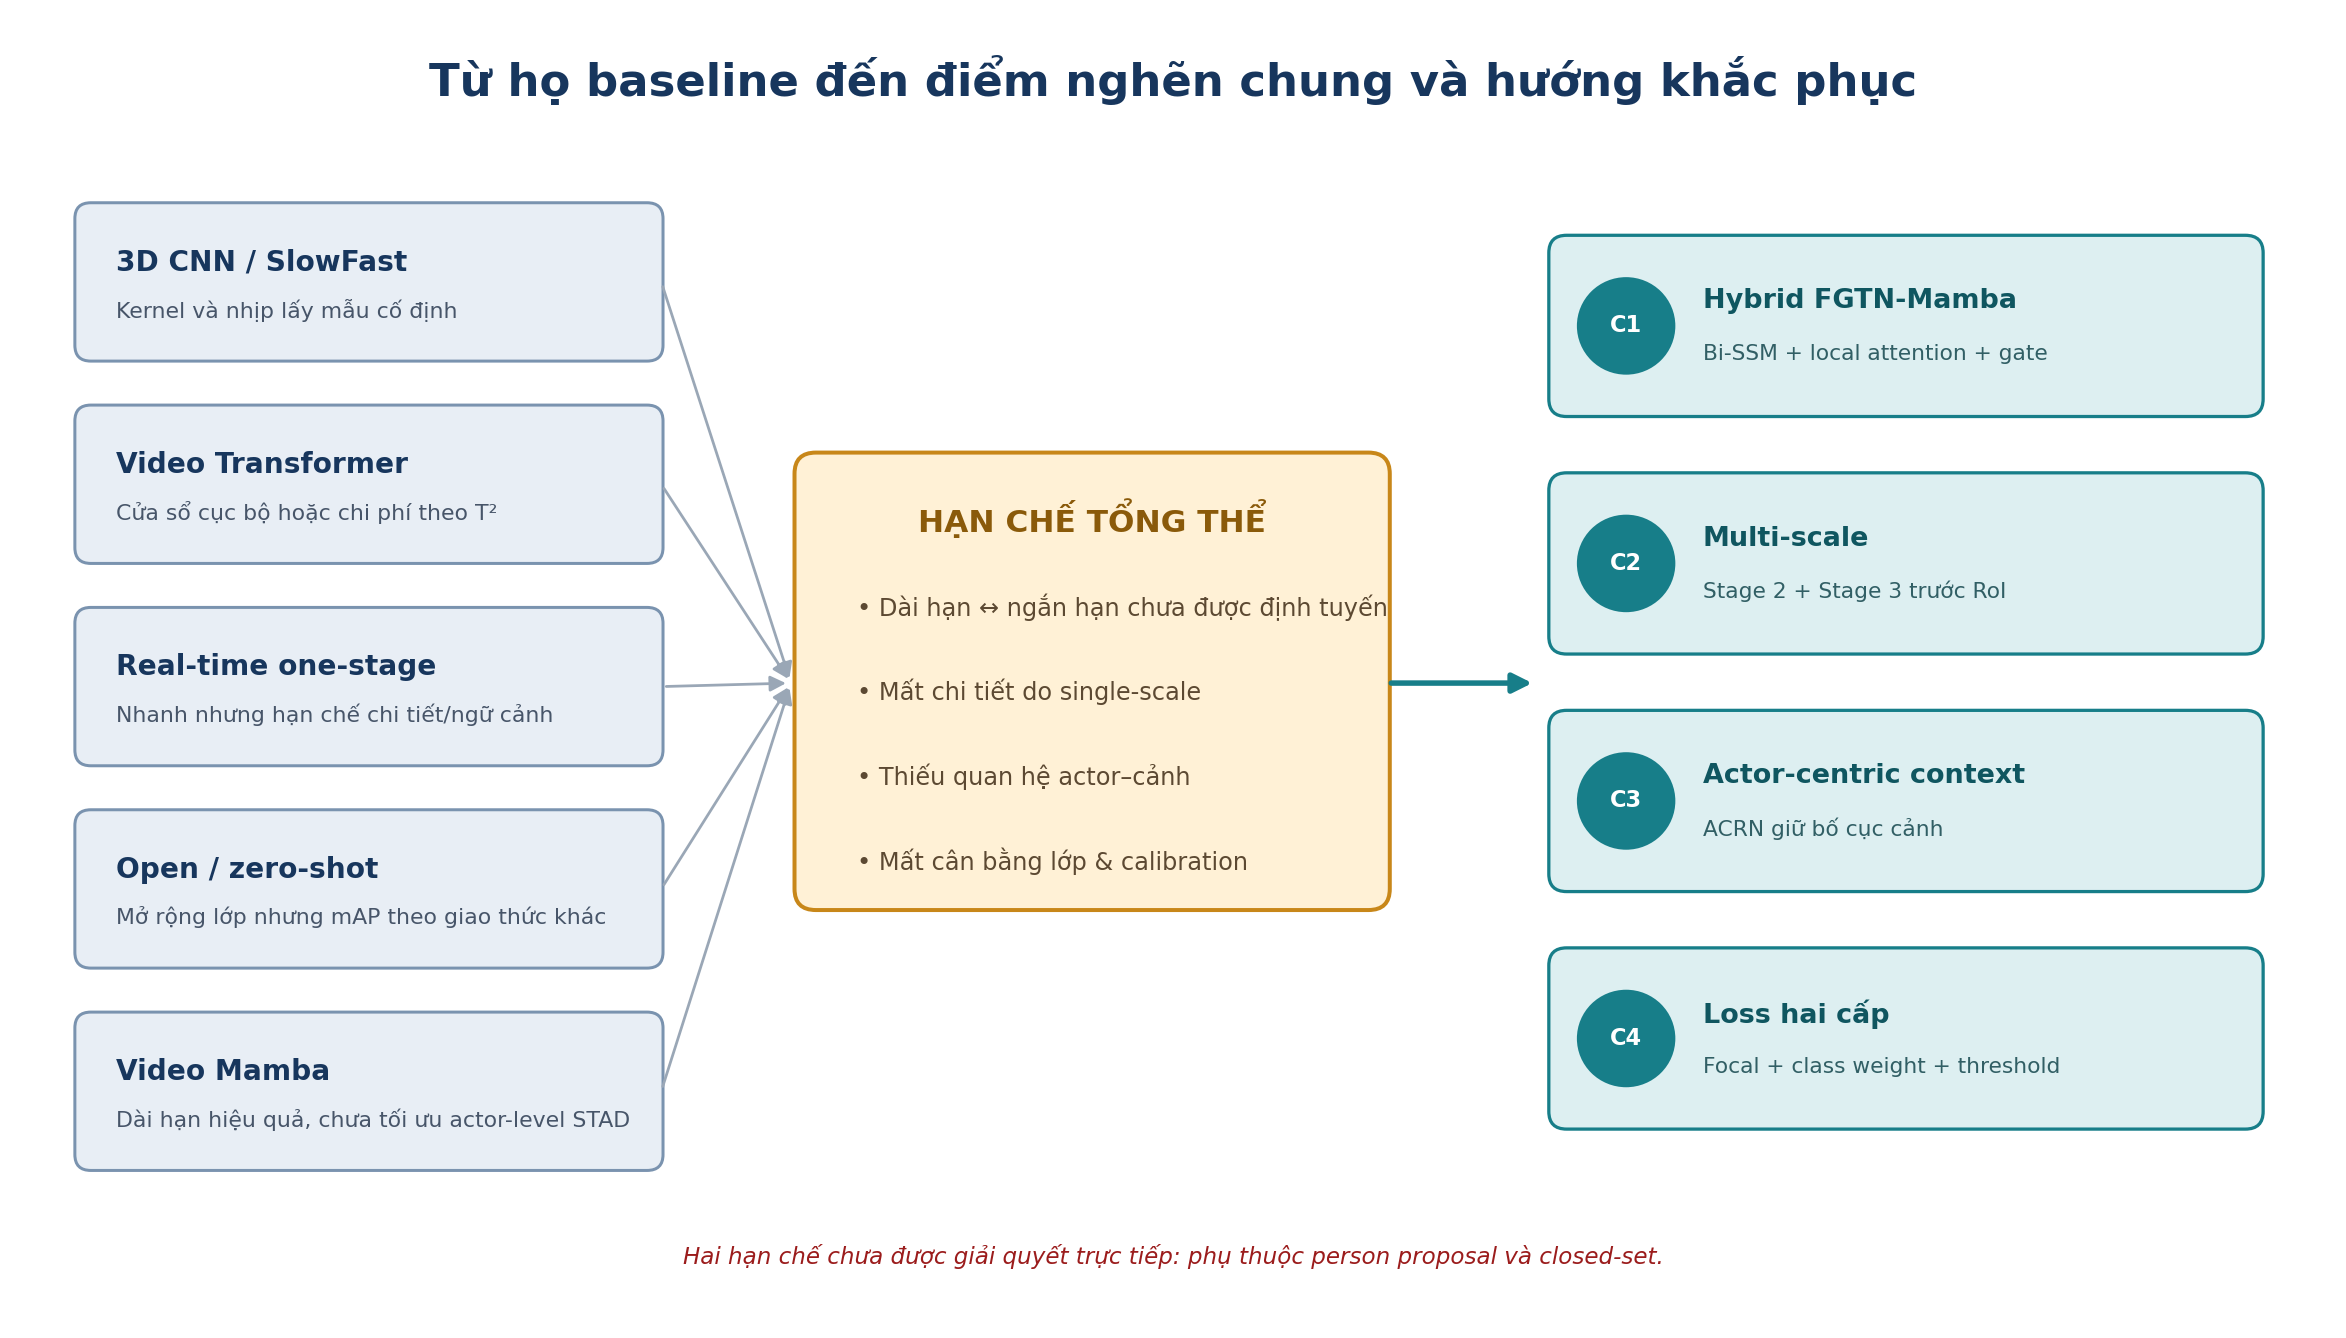
\includegraphics[width=\textwidth]{baseline_gaps.png}
\caption[Từ các họ phương pháp tới hạn chế chung và hướng khắc phục]{Từ các họ phương pháp tới hạn chế chung và bốn hướng khắc phục của luận văn: C1 --- Hybrid FGTN-Mamba (L1, L2); C2 --- đa tỉ lệ (L3); C3 --- ngữ cảnh lấy actor làm trung tâm bằng ACRN (L4); C4 --- hàm mất mát hai cấp và ngưỡng theo lớp (L5).}
\label{fig:gaps}
\end{figure}

\section*{Tiểu kết chương}
\addcontentsline{toc}{section}{Tiểu kết chương}

Chương này đã trình bày cơ sở lý thuyết của attention cửa sổ, mô hình không gian trạng thái chọn lọc, pipeline STAD hai giai đoạn và hàm mất mát cho dữ liệu mất cân bằng. Tổng quan bảy họ phương pháp cho thấy chưa có cơ chế nào vừa truyền ngữ cảnh dài hạn với chi phí tuyến tính, vừa giữ chuyển tiếp ngắn hạn và định tuyến giữa hai thang thời gian theo nội dung tại vị trí tiền-RoI của pipeline STAD theo từng người. Bảy hạn chế L1--L7 được ánh xạ tới các cơ chế xử lý trình bày trong \cref{ch:method}.

\chapter{Hybrid FGTN-Mamba: phương pháp đề xuất}
\label{ch:method}

Chương này mô tả khối Hybrid FGTN-Mamba và pipeline phát hiện hoàn chỉnh. Mọi mô tả bám theo cài đặt trong thư mục \path{projects/fgtn_ava} của kho mã; các siêu tham số nêu dưới đây là giá trị thực tế trong cấu hình huấn luyện.

\section{Tổng quan kiến trúc}
\label{sec:overview}

Pipeline đề xuất (\cref{fig:pipeline}) gồm năm bước:
\begin{enumerate}
  \item Backbone Video Swin-Tiny \cite{liu2022videoswin}, tiền huấn luyện trên Kinetics-400, trích đồng thời bản đồ đặc trưng của tầng 3 và tầng 4.
  \item Mỗi tầng đi qua một Hybrid FGTN-Mamba riêng, với tham số phù hợp độ phân giải và mức ngữ nghĩa của tầng đó, để đặc trưng được làm giàu theo thời gian trước khi cắt theo person proposal.
  \item 3D RoIAlign lấy đặc trưng của từng person proposal ở cả hai tỉ lệ rồi nối theo kênh (multi-scale RoI): tầng 3 giữ chi tiết như điện thoại, bàn tay, bàn chân; tầng 4 giữ ngữ nghĩa toàn thân.
  \item ACRN học quan hệ giữa từng actor với bàn, ghế, thiết bị và cảnh xung quanh.
  \item Head sigmoid dự đoán xác suất độc lập cho từng nhãn, huấn luyện bằng focal loss kết hợp trọng số lớp; khi suy luận, ngưỡng theo lớp và logic theo track giảm cảnh báo chớp tắt.
\end{enumerate}

Thành phần mới trung tâm là Hybrid FGTN-Mamba (bước 2); đặc trưng đa tỉ lệ, ACRN và hàm mất mát hai cấp là các thành phần có tiền lệ, được tích hợp để xử lý các hạn chế còn lại (\cref{sec:multiscale,sec:acrn,sec:loss}). Các tầng của Video Swin-T được đánh số từ 1 đến 4 như \cref{fig:architecture}; tầng 3 và tầng 4 tương ứng \code{out\_indices} 2 và 3 trong mã nguồn (``stage 2'' và ``stage 3'' khi đánh số từ 0). Với đoạn video $V \in \R^{3 \times 32 \times 256 \times 256}$ và $N$ hộp người, chuỗi biến đổi của pipeline đầy đủ là
\begin{equation}
\begin{aligned}
V &\xrightarrow{\text{Swin-T}} \big(F^{(3)}, F^{(4)}\big)
  \xrightarrow{\text{HFM}_3,\ \text{HFM}_4} \big(\tilde{F}^{(3)}, \tilde{F}^{(4)}\big)\\
  &\xrightarrow{\text{RoIAlign}} r_k
  \xrightarrow{\text{ACRN}} c_k
  \xrightarrow{\text{head}} \mat{p}_k \in [0,1]^{K},
\end{aligned}
\label{eq:flow}
\end{equation}
trong đó $F^{(3)} \in \R^{384 \times 16 \times 16 \times 16}$, $F^{(4)} \in \R^{768 \times 16 \times 8 \times 8}$, $\text{HFM}_s$ là ngăn xếp hai khối Hybrid FGTN-Mamba của tầng $s$, $r_k \in \R^{1152 \times 1 \times 8 \times 8}$ là đặc trưng RoI đa tỉ lệ và $c_k$ là đầu ra của ACRN. Biến thể một tỉ lệ (cấu hình A6 trong \cref{tab:ablation}) bỏ tầng 3 và ACRN: $V \rightarrow F^{(4)} \rightarrow \tilde{F}^{(4)} \rightarrow r_k \in \R^{768 \times 1 \times 8 \times 8} \rightarrow \mat{p}_k$.

\begin{figure}[H]
\centering
\resizebox{\textwidth}{!}{%
\begin{tikzpicture}[font=\footnotesize, >={Stealth[length=2mm]},
  blk/.style={draw, rounded corners=2pt, align=center, inner sep=3pt,
              minimum height=10mm, line width=0.6pt},
  arr/.style={->, line width=0.7pt}]
  \node[blk, fill=blue!7, minimum width=17mm, minimum height=32mm] (swin)
    {Video\\Swin-T\\[3pt]{\scriptsize tiền huấn}\\{\scriptsize luyện K400}};
  \node[blk, fill=orange!14, minimum width=29mm, anchor=west] (h3)
    at ($(swin.east)+(21mm,9mm)$) {Hybrid FGTN-Mamba\\{\scriptsize tham số riêng tầng 3}};
  \node[blk, fill=orange!14, minimum width=29mm, anchor=west] (h4)
    at ($(swin.east)+(21mm,-9mm)$) {Hybrid FGTN-Mamba\\{\scriptsize tham số riêng tầng 4}};
  \draw[arr] ($(swin.east)+(0,9mm)$) --
    node[above, font=\scriptsize] {tầng 3}
    node[below, font=\scriptsize] {$C{=}384$, $\tfrac{1}{16}$} (h3.west);
  \draw[arr] ($(swin.east)+(0,-9mm)$) --
    node[above, font=\scriptsize] {tầng 4}
    node[below, font=\scriptsize] {$C{=}768$, $\tfrac{1}{32}$} (h4.west);
  \coordinate (mid) at ($(h3.east)!0.5!(h4.east)$);
  \node[blk, fill=green!10, minimum width=22mm, anchor=west] (roi) at ($(mid)+(10mm,0)$)
    {RoIAlign 3D\\đa tỉ lệ\\{\scriptsize nối kênh $384{+}768$}};
  \draw[arr] (h3.east) -- ++(5mm,0) |- ($(roi.west)+(0,2.5mm)$);
  \draw[arr] (h4.east) -- ++(5mm,0) |- ($(roi.west)+(0,-2.5mm)$);
  \node[blk, fill=gray!8, above=6mm of roi] (prop) {Person proposal};
  \draw[arr] (prop) -- (roi);
  \node[blk, fill=green!10, right=6mm of roi] (acrn) {ACRN\\{\scriptsize actor--cảnh}};
  \node[blk, fill=magenta!8, right=6mm of acrn] (head) {Head\\sigmoid\\{\scriptsize đa nhãn}};
  \node[blk, fill=gray!8, right=6mm of head] (alert) {Ngưỡng theo lớp\\+ logic theo track\\$\Rightarrow$ cảnh báo};
  \draw[arr] (roi) -- (acrn);
  \draw[arr] (acrn) -- (head);
  \draw[arr] (head) -- (alert);
\end{tikzpicture}}
\caption[Pipeline phát hiện đầy đủ]{Pipeline phát hiện đầy đủ: Video Swin-T trích đặc trưng tầng 3 (384 kênh, bước 16) và tầng 4 (768 kênh, bước 32); mỗi tầng qua một Hybrid FGTN-Mamba với tham số riêng; RoIAlign 3D lấy đặc trưng của từng person proposal ở hai tỉ lệ và nối theo kênh; ACRN bổ sung quan hệ actor--cảnh; head sigmoid cho điểm từng hành vi; ngưỡng theo lớp và logic theo track quyết định việc phát cảnh báo.}
\label{fig:pipeline}
\end{figure}

\begin{figure}[htbp]
\centering
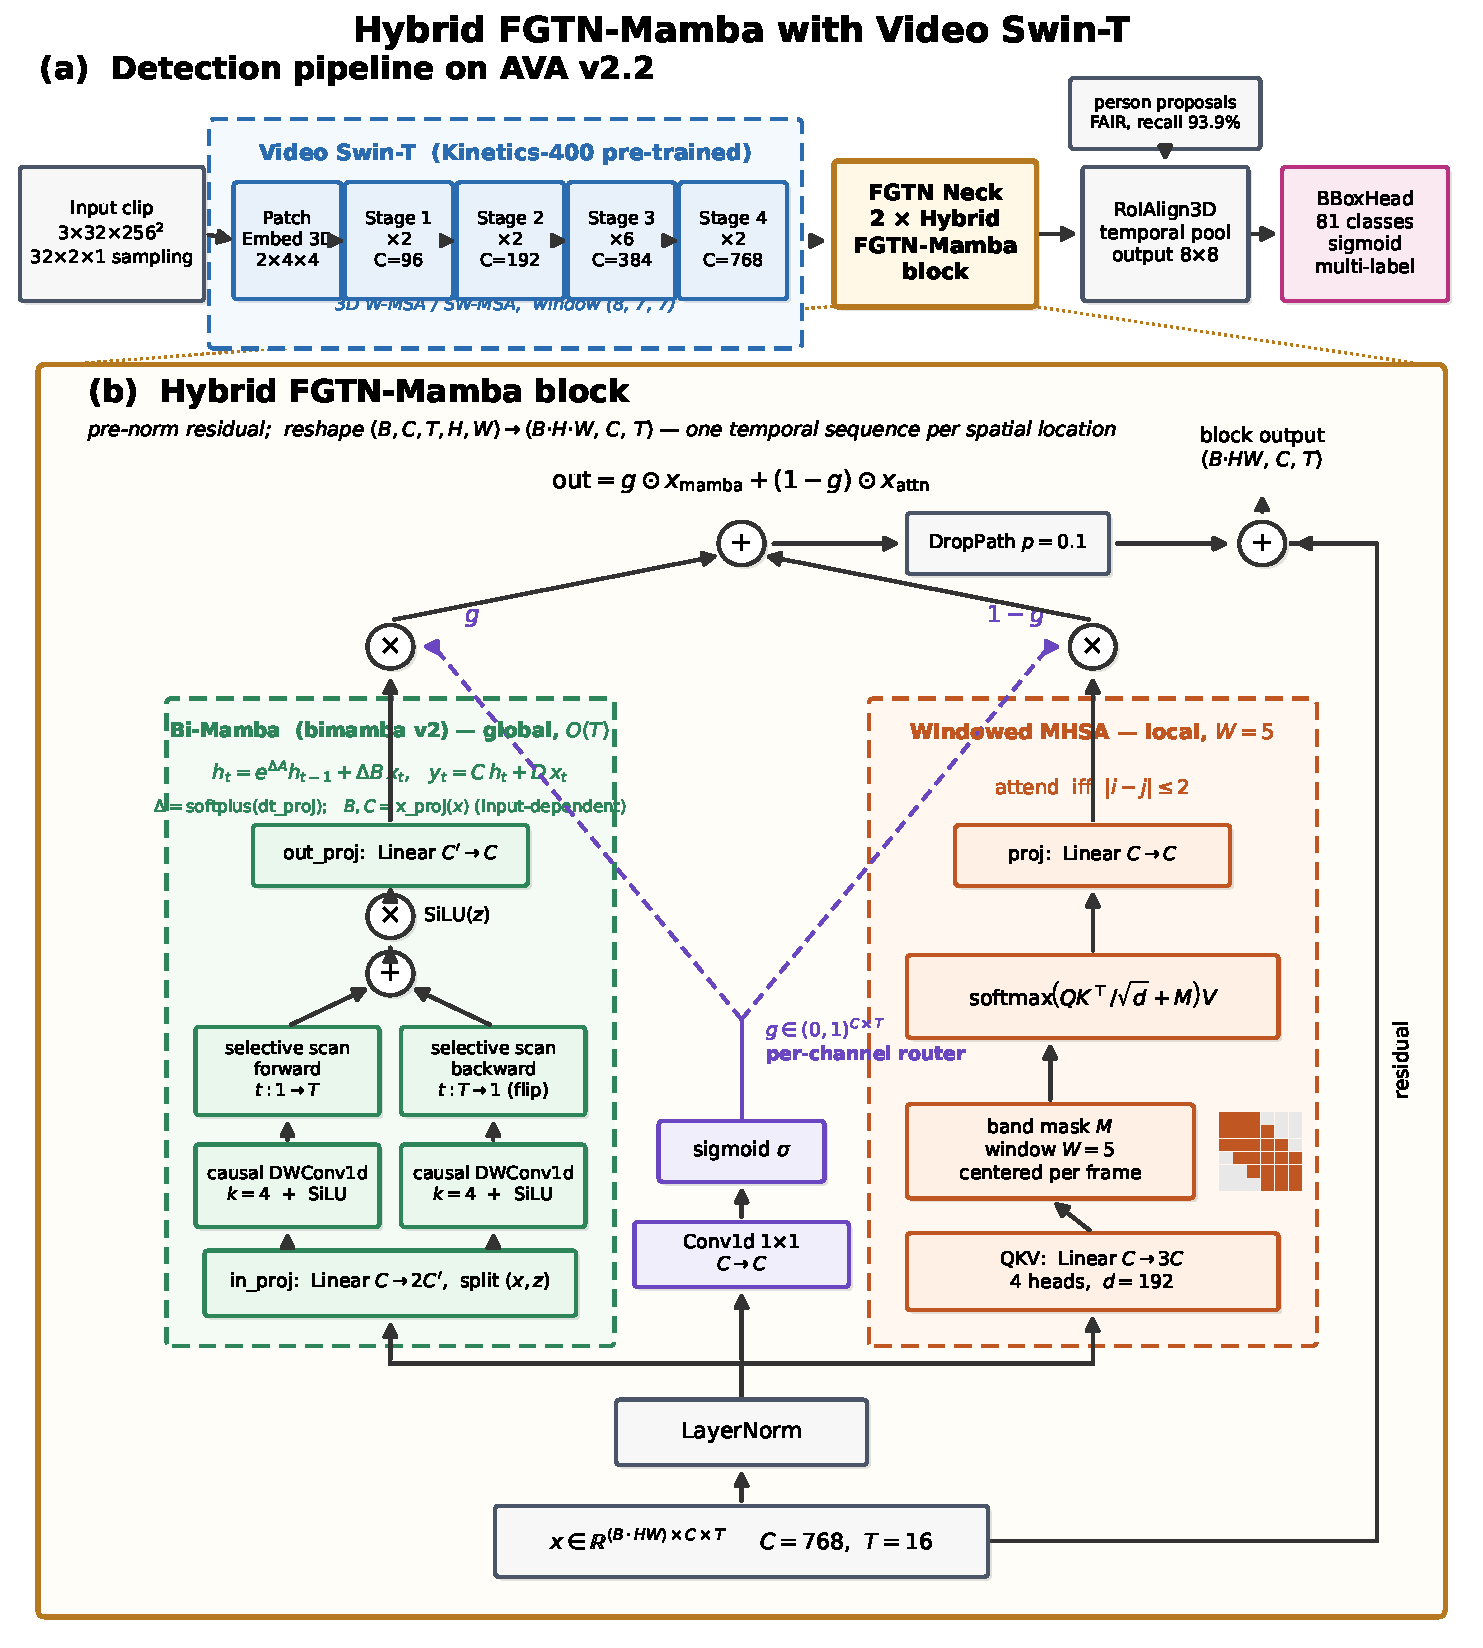
\includegraphics[width=\textwidth]{fgtn_architecture.pdf}
\caption[Biến thể một tỉ lệ và cấu trúc khối Hybrid FGTN-Mamba]{Biến thể một tỉ lệ và cấu trúc khối. (a) Pipeline một tỉ lệ: Video Swin-T $\rightarrow$ FGTN neck (hai khối Hybrid FGTN-Mamba) $\rightarrow$ RoIAlign3D $\rightarrow$ BBoxHead sigmoid đa nhãn; pipeline đầy đủ bổ sung nhánh tầng 3 và ACRN như \cref{fig:pipeline}. (b) Một khối Hybrid FGTN-Mamba: nhánh Bi-Mamba (selective scan hai chiều, $O(T)$), nhánh windowed MHSA (mặt nạ dải, $W = 5$) và cổng sigmoid theo kênh và bước thời gian, $\mathrm{out} = g \odot x_{\text{mamba}} + (1 - g) \odot x_{\text{attn}}$.}
\label{fig:architecture}
\end{figure}

\section{Vị trí đặt khối: hậu-backbone, tiền-RoI}
\label{sec:placement}

Khối được đặt sau backbone và trước 3D RoIAlign vì ba lý do. Nếu đặt bên trong Video Swin, phải sửa kiến trúc đã tiền huấn luyện và trọng số Kinetics-400 không còn nạp được nguyên vẹn. Nếu đặt sau RoIAlign, mô hình thời gian chỉ nhìn vùng người đã bị cắt, mất tín hiệu cảnh; hơn nữa \code{SingleRoIExtractor3D} gộp trung bình theo thời gian trước khi cắt nên trục $T$ không còn sau RoI. Khi đặt tiền-RoI, mỗi vị trí không gian được làm giàu bằng lịch sử dọc trục thời gian rồi RoIAlign mới lấy phần liên quan đến từng actor; giao diện ``tensor vào, tensor cùng kích thước ra'' cho phép thay backbone mà không đổi neck. Vị trí này cũng xác định phạm vi cải tiến: khối cải thiện biểu diễn theo thời gian, không sửa lỗi của person proposal và không tự giải quyết mất cân bằng dữ liệu.

\section{Đầu vào, định dạng lại và chuẩn hóa}
\label{sec:reshape}

Với bản đồ đặc trưng $F \in \R^{B \times C \times T \times H \times W}$, neck chỉ mô hình hóa dọc trục $T$, không trộn không gian thêm lần nữa. Tensor được hoán vị và định dạng lại thành
\begin{equation}
\mat{X} = \mathrm{reshape}\big(\mathrm{permute}(F)\big) \in \R^{(B \cdot H \cdot W) \times C \times T},
\label{eq:reshape}
\end{equation}
tức mỗi tọa độ không gian là một chuỗi độc lập gồm $T$ token $C$ chiều; sau các khối, tensor được đưa về dạng ban đầu. Mỗi khối dùng chuẩn hóa trước (pre-norm) trên chiều kênh tại từng bước thời gian:
\begin{equation}
\bar{\mat{X}} = \LN(\mat{X}), \qquad \epsilon = 10^{-6}.
\label{eq:prenorm}
\end{equation}
Ở tầng 4, $C = 768$, $T = 16$ (32 khung hình qua patch embedding thời gian bước 2), $H = W = 8$ và số chuỗi là $B \cdot 64$; ở tầng 3, $C = 384$, $H = W = 16$ và số chuỗi là $B \cdot 256$.

\section{Nhánh toàn cục: mô hình không gian trạng thái chọn lọc hai chiều}
\label{sec:ssm-branch}

Nhánh SSM nhắm vào L1 và L2 (\cref{tab:gaps}). Với hành vi bền vững như ngủ trên bàn hay gác chân, vài khung hình quanh khung hình khóa không đủ để phân biệt tư thế tạm thời với hành vi kéo dài; selective scan truyền một trạng thái qua toàn bộ chuỗi với số bước tuyến tính theo $T$. Nhánh dùng khối Mamba \cite{gu2023mamba} theo cài đặt \code{bimamba v2} của Video Mamba Suite \cite{chen2024videomambasuite}, với $N = 16$, hệ số mở rộng $E = 2$ ($C' = 2C$), hạng phép chiếu bước thời gian $\lceil C/16 \rceil$ và tích chập nhân quả theo kênh $k = 4$. Trên mỗi chuỗi $\bar{\mat{X}} \in \R^{T \times C}$:
\begin{align}
[\mat{U};\ \mat{Z}] &= \bar{\mat{X}}\mat{W}_{\text{in}}, \qquad \mat{U}, \mat{Z} \in \R^{T \times C'}, \label{eq:mamba-in}\\
\mat{U}' &= \mathrm{SiLU}\big(\mathrm{DWConv1d}_{k=4}(\mat{U})\big), \label{eq:mamba-conv}\\
\Delta_t &= \mathrm{softplus}\big(\mat{W}_\Delta \mat{W}_{\text{dt}} \mat{u}'_t + \mat{b}_\Delta\big), \quad
\mat{B}_t = \mat{W}_B \mat{u}'_t, \quad \mat{C}_t = \mat{W}_C \mat{u}'_t, \label{eq:mamba-sel}\\
\mat{h}_t &= \exp(\Delta_t \mat{A})\,\mat{h}_{t-1} + \Delta_t \mat{B}_t \mat{u}'_t, \qquad
y_t = \mat{C}_t^{\top}\mat{h}_t + D\,u'_t, \label{eq:mamba-scan}\\
\mat{S}^{\rightarrow} &= \mat{Y} \odot \mathrm{SiLU}(\mat{Z}). \label{eq:mamba-gate}
\end{align}
Ở đây $\mat{A} = -\exp(\mat{A}_{\log})$ là tham số học được, còn $\Delta_t$, $\mat{B}_t$, $\mat{C}_t$ sinh từ đầu vào tại mỗi bước, nên mức giữ/quên trạng thái thay đổi theo nội dung: đoạn gần như tĩnh duy trì trạng thái lâu hơn, thay đổi đột ngột làm tăng trọng số cho đầu vào mới. Tính chọn lọc này quan trọng hơn việc chỉ thay attention bằng một phép hồi quy, và phù hợp với dữ liệu có cả hành vi bền vững lẫn thao tác nhanh. Vì đoạn video lấy đối xứng quanh khung hình khóa, \code{bimamba v2} dùng thêm một bộ tham số quét riêng cho chiều ngược, dùng chung $\mat{W}_{\text{in}}$ và $\mat{W}_{\text{out}}$:
\begin{equation}
\mat{S}^{\leftarrow} = \mathrm{flip}\big(\Scan_b(\mathrm{flip}(\bar{\mat{X}}))\big), \qquad
\mat{S} = \tfrac{1}{2}\big(\mat{S}^{\rightarrow} + \mat{S}^{\leftarrow}\big)\mat{W}_{\text{out}} \in \R^{T \times C}.
\label{eq:bimamba}
\end{equation}
Quét ngược bổ sung các khung hình sau khung hình khóa, đổi lại hệ cảnh báo trực tuyến phải chịu độ trễ nhìn trước (look-ahead) tương ứng (\cref{sec:inference}).

\section{Nhánh cục bộ: self-attention trong cửa sổ thời gian}
\label{sec:local-branch}

SSM nén lịch sử vào trạng thái nên có thể làm mờ một chuyển tiếp rất ngắn, như pha đưa điện thoại lên hay bắt đầu một thao tác nguy hiểm. Nhánh cục bộ giữ đường so khớp trực tiếp giữa mỗi khung hình và các khung hình lân cận. Từ $\bar{\mat{X}}$, phép chiếu $\mat{W}_{\text{qkv}} \in \R^{C \times 3C}$ tạo $\mat{Q}, \mat{K}, \mat{V}$ chia thành $h = 4$ đầu; với $W = 5$, token $i$ chỉ chú ý tới token $j$ thỏa $|i - j| \leq 2$:
\begin{equation}
\mat{A}_{\text{loc}} = \softmax\!\left(\frac{\mat{Q}\mat{K}^{\top}}{\sqrt{d}} + \mat{M}\right)\mat{V}\,\mat{W}_{\text{proj}}, \qquad
M_{ij} = \begin{cases} 0, & |i - j| \leq 2,\\ -\infty, & \text{ngược lại.}\end{cases}
\label{eq:local-attn}
\end{equation}
Ở biên đoạn video, mặt nạ chỉ giữ các phần tử hợp lệ, không quấn vòng; bốn đầu cho phép các không gian con kênh học các kiểu chuyển động khác nhau. Vì $T = 16$ tại neck, ma trận $T \times T$ được tính rồi che với chi phí không đáng kể; khi $T$ lớn, cùng công thức có thể thực thi theo dạng dải với chi phí $O(TWC)$ \cite{beltagy2020longformer}. Nhánh cục bộ chưa dùng mã hóa vị trí tương đối; thứ tự thời gian được nhánh SSM cung cấp gián tiếp qua đường residual.

\section{Cổng sigmoid: định tuyến dài hạn--ngắn hạn theo nội dung}
\label{sec:gate}

Nếu cộng $\mat{S}$ và $\mat{A}_{\text{loc}}$ với trọng số cố định, mọi kênh và mọi đoạn video nhận cùng tỷ lệ dài hạn--ngắn hạn, mâu thuẫn với đặc thù các hành vi ở \cref{sec:behaviours}. Cổng sigmoid là bộ định tuyến mềm, tính từ đầu vào đã chuẩn hóa bằng tích chập $1 \times 1$ theo kênh:
\begin{equation}
\mat{G} = \sigma\big(\mat{W}_g \bar{\mat{X}} + \mat{b}_g\big) \in (0,1)^{C \times T}, \qquad
\mat{Z} = \mat{G} \odot \mat{S} + (\mat{1} - \mat{G}) \odot \mat{A}_{\text{loc}}.
\label{eq:gate}
\end{equation}
Cổng phụ thuộc nội dung, vị trí không gian, kênh và bước thời gian: cùng một kênh có thể ưu tiên trạng thái dài hạn ở pha tĩnh và chuyển sang nhánh cục bộ tại thời điểm chuyển tiếp; vì không chọn cứng, gradient vẫn truyền qua cả hai nhánh. Đầu ra khối là
\begin{equation}
\mat{Y} = \mat{X} + \mathrm{DropPath}_{p = 0{,}1}(\mat{Z}),
\label{eq:residual}
\end{equation}
với DropPath \cite{huang2016droppath} loại bỏ ngẫu nhiên toàn bộ nhánh dư của một chuỗi trong lúc huấn luyện; hai khối như vậy được xếp chồng.

Cùng một module cài đặt bốn chế độ qua tham số \code{branch\_mode}, phục vụ phần lớn ma trận ablation (\cref{tab:ablation}): \code{hybrid} theo \cref{eq:gate} (A6); \code{no\_gate} với $\mat{Z} = 0{,}5\,\mat{S} + 0{,}5\,\mat{A}_{\text{loc}}$ (A5); \code{mamba\_only} với $\mat{Z} = \mat{S}$ (A3); \code{attn\_only} với $\mat{Z} = \mat{A}_{\text{loc}}$ (A4). Temporal MHSA toàn cục (A1) là trường hợp riêng của \code{attn\_only} khi cửa sổ phủ toàn đoạn (\code{window\_size} $\geq 31$ với $T = 16$); baseline không neck (A0) tương ứng \code{model.neck = None}; SSM một chiều (A2) dùng \code{bimamba\_type = "none"} của \code{mamba-ssm}, hiện chưa có khóa cấu hình tương ứng.

\section{Ổn định huấn luyện và cài đặt dự phòng}
\label{sec:stability}

Pre-norm và residual cho phép khối học phần dư thay vì tái tạo toàn bộ bản đồ đặc trưng; ở khởi tạo, hai nhánh đóng góp nhỏ và pipeline xấp xỉ pipeline không có neck, nên trọng số tiền huấn luyện của backbone không bị phá vỡ. Gradient được cắt với chuẩn tối đa 40 theo công thức gốc của MMAction2 cho AVA; kernel selective scan CUDA của \code{mamba-ssm} được khóa phiên bản vì sai khác kernel có thể ảnh hưởng tốc độ và khả năng tái lập. Khi thư viện \code{mamba-ssm} không khả dụng (ví dụ kiểm thử trên CPU), mã nguồn cung cấp bản cài đặt thuần PyTorch \code{NaiveBiMamba} thực hiện đúng hồi quy \cref{eq:mamba-scan} bằng vòng lặp theo $T$ với hai bộ tham số xuôi/ngược; bản này tương đương về mặt số học nhưng chậm hơn khoảng hai bậc, chỉ dùng để kiểm tra kích thước tensor.

\section{Độ phức tạp và so sánh với các temporal neck khác}
\label{sec:complexity}

Xét chuỗi độ dài $T$, $C$ kênh, cửa sổ $W$, trạng thái $N$ và hệ số mở rộng $E$. Trong một khối, nhánh SSM tốn $O(T \cdot C \cdot EC)$ cho các phép chiếu, $O(T \cdot EC \cdot k)$ cho tích chập và $O(T \cdot EC \cdot N)$ cho selective scan mỗi chiều; nhánh cục bộ tốn $O(T \cdot C^2)$ cho phép chiếu và $O(T \cdot W \cdot C)$ cho so khớp trong cửa sổ; cổng tốn $O(T \cdot C^2)$. Mọi số hạng đều tuyến tính theo $T$: tổng chi phí là $O\big(T(C^2 + CN + WC)\big)$ và phần phụ thuộc cấu trúc thời gian là $O(TC + TWC)$, thay vì $O(T^2 C)$ của attention toàn cục (\cref{tab:necks}). Chi phí toàn neck nhân với số chuỗi $B \cdot H \cdot W$, nên tầng 3 ($16 \times 16$) tốn gấp bốn lần tầng 4.

\begin{table}[htbp]
\centering
\caption{So sánh các temporal neck tại cùng vị trí hậu-backbone}
\label{tab:necks}
\small
\begin{tabularx}{\textwidth}{lXlX}
\toprule
\textbf{Cơ chế} & \textbf{Nội dung} & \textbf{Chi phí theo $T$} & \textbf{Đặc tính}\\
\midrule
Temporal MHSA toàn cục & So khớp mọi cặp khung hình & $O(T^2 C)$ & Toàn cục nhưng bộ nhớ tăng nhanh\\
Tích chập thời gian / TPN \cite{yang2020tpn} & Nhân, hệ số giãn cố định & $O(T k C^2)$ & Thiên lệch cục bộ; trường tiếp nhận theo độ sâu\\
SSM thuần \cite{li2024videomamba} & Selective scan & $O(TC)$ & Dài hạn tốt; có thể thiếu chuyển tiếp cục bộ\\
Hybrid FGTN-Mamba & Bi-SSM + W-MHSA + cổng & $O(TC + TWC)$ & Dài--ngắn tách nhánh, định tuyến theo nội dung\\
\bottomrule
\end{tabularx}
\end{table}

\Cref{tab:params} tổng hợp số tham số theo cấu trúc của neck. Với $C = 768$, một khối có 6.957.312 tham số (nhánh Mamba 4.002.816, nhánh attention 2.362.368, cổng 590.592); neck hai khối có 13.914.624 tham số, khoảng một nửa backbone Video Swin-T (27.850.470). Pipeline đầy đủ thêm khoảng 3,57 triệu tham số cho ngăn xếp tầng 3 và khoảng 14,6 triệu cho ACRN. Ngoài chi phí tuyến tính, khối đưa vào ba thiên lệch quy nạp phù hợp bài toán: trạng thái có thứ tự cho diễn biến dài, so khớp cục bộ cho chuyển tiếp ngắn và bộ định tuyến theo nội dung.

\begin{table}[htbp]
\centering
\caption{Số tham số theo cấu trúc của neck một tỉ lệ ($C = 768$, hai khối)}
\label{tab:params}
\begin{tabularx}{\textwidth}{Xrr}
\toprule
\textbf{Thành phần (mỗi khối)} & \textbf{Kích thước chính} & \textbf{Tham số}\\
\midrule
LayerNorm & $2 \times 768$ & 1.536\\
Mamba: \code{in\_proj} & $3072 \times 768$ & 2.359.296\\
Mamba: hai bộ quét (conv1d, \code{x\_proj}, \code{dt\_proj}, $\mat{A}_{\log}$, $D$) & $2 \times 231.936$ & 463.872\\
Mamba: \code{out\_proj} & $768 \times 1536$ & 1.179.648\\
W-MHSA: \code{qkv} + \code{proj} & $2304 \times 768$, $768 \times 768$ & 2.362.368\\
Cổng: Conv1d $1 \times 1$ & $768 \times 768$ & 590.592\\
\midrule
Một khối & & 6.957.312\\
Neck (hai khối) & & 13.914.624\\
\bottomrule
\end{tabularx}
\end{table}

\section{Thành phần tích hợp 1: đặc trưng đa tỉ lệ}
\label{sec:multiscale}

Thành phần này xử lý L3. Video Swin-T tạo bốn tầng đặc trưng với $96, 192, 384, 768$ kênh và bước giảm mẫu $4, 8, 16, 32$. Chỉ dùng tầng 4 thì điện thoại hay bàn chân chiếm chưa đến một ô trên lưới $8 \times 8$. Pipeline đầy đủ đặt \code{out\_indices = (2, 3)} để lấy thêm tầng 3 và tạo \emph{một ngăn xếp Hybrid FGTN-Mamba riêng cho mỗi tầng} (\code{in\_channels = (384, 768)}), không chia sẻ tham số. Sau neck, \code{SingleRoIExtractor3D} nội suy bản đồ tầng 4 về độ phân giải tầng 3, gộp trung bình theo thời gian, nối theo kênh và cắt RoI với tỷ lệ $1/16$:
\begin{equation}
r_k = \RoIAlign\Big(\Concat\big[\Pool_T(\tilde{F}^{(3)}),\ \Pool_T(\uparrow_2 \tilde{F}^{(4)})\big],\ b_k\Big) \in \R^{1152 \times 1 \times 8 \times 8}.
\label{eq:multiscale}
\end{equation}
Gộp theo thời gian được thực hiện có chủ đích \emph{sau} khi mỗi tầng đã nhận ngữ cảnh dài--ngắn từ neck. Tầng 3 có số chuỗi thời gian gấp bốn tầng 4, nên kích thước lô của cấu hình đa tỉ lệ cần được lựa chọn theo bộ nhớ khả dụng; cặp A6 $\rightarrow$ A7 tách đóng góp của thành phần này.

\section{Thành phần tích hợp 2: mạng quan hệ actor--cảnh (ACRN)}
\label{sec:acrn}

ACRN \cite{sun2018acrn} xử lý L4: trong phân xưởng, cùng một tư thế mang ý nghĩa khác nhau tùy theo bàn, ghế, thiết bị xung quanh người. Luận văn dùng \code{ACRNHead} của MMAction2 làm \code{shared\_head} trong \code{AVARoIHead}. Với đặc trưng RoI $r_k$ và bản đồ cảnh $G$ (đã gộp theo thời gian, $1152 \times 1 \times h \times w$):
\begin{multline}
c_k = \mathrm{Conv}_{1\times3\times3}\Big(\mathrm{Conv}_{1\times1\times1}\big(\Concat[\Tile_{h \times w}(\max\!\Pool(r_k)),\ G_{\text{batch}(k)}]\big)\Big)\\
\in \R^{1152 \times 1 \times h \times w},
\label{eq:acrn}
\end{multline}
trong đó mỗi tích chập kèm BatchNorm và ReLU. Vectơ actor được lát (tile) lên toàn bộ lưới cảnh, nên quan hệ được điều kiện theo từng actor: hai người trong cùng khung hình nhận ngữ cảnh khác nhau. So với gộp trung bình toàn cục, ACRN giữ bố cục không gian của cảnh; so với STAR \cite{gritsenko2024star}, nó vẫn phụ thuộc proposal nhưng tích hợp trực tiếp vào pipeline hai giai đoạn.

\section{Thành phần tích hợp 3: hàm mất mát hai cấp và ngưỡng theo lớp}
\label{sec:loss}

Head \code{BBoxHeadAVA} của MMAction2 chỉ giữ các RoI có ít nhất một nhãn dương ($\mathcal{P}$) và tính BCE trên $K$ logit sigmoid:
\begin{equation}
\mathcal{L}_{\text{BCE}} = \frac{1}{|\mathcal{P}| \cdot K} \sum_{k \in \mathcal{P}} \sum_{c=1}^{K}
  \BCE\big(s_{k,c}, y_{k,c}\big).
\label{eq:bce}
\end{equation}
Thành phần này xử lý L5: head \code{BBoxHeadAVAWeighted} giữ nguyên phần chọn RoI và chỉ thay biểu thức mất mát bằng focal loss có trọng số lớp,
\begin{equation}
\begin{gathered}
\mathcal{L} = \frac{1}{|\mathcal{P}| \cdot K} \sum_{k \in \mathcal{P}} \sum_{c=1}^{K}
  w_c\, \alpha\, (1 - p_{t,k,c})^{\gamma}\, \BCE(s_{k,c}, y_{k,c}),\\
p_{t,k,c} = \exp\big(-\BCE(s_{k,c}, y_{k,c})\big),
\end{gathered}
\label{eq:focal}
\end{equation}
với $\gamma = 2$, $\alpha = 1$; khi $\gamma = 0$ và $w_c = 1$, \cref{eq:focal} trùng với \cref{eq:bce}. Trọng số lớp tính theo số mẫu hiệu dụng \cite{cui2019classbalanced}:
\begin{equation}
w_c = \frac{\tilde{w}_c}{\frac{1}{K}\sum_{c'} \tilde{w}_{c'}}, \qquad
\tilde{w}_c = \frac{1 - \beta}{1 - \beta^{\max(n_c, 1)}}, \qquad \beta = 0{,}999,
\label{eq:classweight}
\end{equation}
được chuẩn hóa để trung bình bằng 1 và cắt trên tại 10. Sau huấn luyện, ngưỡng $\tau_c$ của từng lớp được chọn trên tập kiểm định theo tiêu chí nghiệp vụ (ví dụ cực đại F1 hoặc đạt recall tối thiểu); mAP không phụ thuộc ngưỡng nên không bị ảnh hưởng bởi lựa chọn này.

\section{Luồng suy luận và logic cảnh báo}
\label{sec:inference}

\begin{enumerate}
  \item Lấy đoạn 32 khung hình (bước 2) đối xứng quanh khung hình khóa, đổi kích thước cạnh ngắn về 256; đọc person proposal (hoặc chạy bộ phát hiện người).
  \item Trích đặc trưng tầng 3 và tầng 4, chạy Hybrid FGTN-Mamba riêng trên từng tầng, 3D RoIAlign đa tỉ lệ, ACRN và head sigmoid cho $p_{k,c}$.
  \item So $p_{k,c}$ với $\tau_c$; chỉ phát sự kiện khi cùng actor vượt ngưỡng $m$ trong $n$ khung hình khóa liên tiếp, giảm cảnh báo chớp tắt.
  \item Ghép sự kiện theo định danh track, lưu thời điểm, hộp, lớp, điểm và ảnh minh chứng; áp dụng thời gian chờ (cooldown) để tránh lặp cảnh báo.
\end{enumerate}
Các tham số $m/n$, cooldown và $\tau_c$ thuộc lớp nghiệp vụ, không được tối ưu trên tập kiểm tra. Độ trễ đầu--cuối gồm giải mã, bộ phát hiện người, bộ đệm nhìn trước của quét hai chiều (tối thiểu nửa đoạn video), mô hình và gửi cảnh báo; thời gian suy luận của riêng mô hình không đại diện cho toàn hệ thống. \Cref{tab:shapes} tóm tắt kích thước tensor qua pipeline.

\begin{table}[H]
\centering
\caption{Chuỗi kích thước đặc trưng với ảnh cắt $256 \times 256$, 32 khung hình đầu vào}
\label{tab:shapes}
\small
\begin{tabularx}{\textwidth}{llX}
\toprule
\textbf{Khối} & \textbf{Kích thước} & \textbf{Ghi chú}\\
\midrule
Đầu vào & $B \times 3 \times 32 \times 256 \times 256$ & Đoạn RGB\\
Patch embedding $(2, 4, 4)$ & $B \times 96 \times 16 \times 64 \times 64$ & $T = 16$ từ đây\\
Swin tầng 3 & $B \times 384 \times 16 \times 16 \times 16$ & Chỉ trong pipeline đa tỉ lệ\\
Swin tầng 4 & $B \times 768 \times 16 \times 8 \times 8$ & Cả hai biến thể\\
Neck (mỗi tầng) & giữ nguyên kích thước & Mô hình hóa thời gian theo từng vị trí\\
RoI tầng 4 (một tỉ lệ) & $N \times 768 \times 1 \times 8 \times 8$ & Gộp trung bình theo $T$ trước khi cắt\\
RoI đa tỉ lệ & $N \times 1152 \times 1 \times 8 \times 8$ & Nối $384 + 768$ tại tỷ lệ $1/16$\\
ACRN & $N \times 1152 \times 1 \times 16 \times 16$ & Lưới cảnh tầng 3\\
Head & $N \times (K + 1)$ & $K$ lớp $+$ nền ($K = 4$ hoặc 80)\\
\bottomrule
\end{tabularx}
\end{table}

\section{Rủi ro kỹ thuật và cách giám sát}
\label{sec:risks}

\begin{itemize}
  \item \emph{Cổng bão hòa}: $g$ dồn về một nhánh; theo dõi phân bố $g$ và chuẩn gradient từng nhánh theo epoch.
  \item \emph{Tầng lấn át}: tầng 4 lấn tầng 3 trong cấu hình đa tỉ lệ; đo chuẩn đặc trưng và ablation từng tầng.
  \item \emph{Điểm nóng bộ nhớ}: tầng 3 tạo $B \cdot 256$ chuỗi; theo dõi bộ nhớ đỉnh theo lô, $T$ và độ phân giải.
  \item \emph{Độ trễ hai chiều}: quét ngược cần khung hình tương lai; báo cả thông lượng và độ trễ đầu--cuối.
  \item \emph{Sai lệch tỷ lệ RoI}: \code{featmap\_stride} của bộ trích RoI phải khớp bước giảm mẫu của bản đồ đặc trưng (32 với tầng 4, 16 với cấu hình đa tỉ lệ).
  \item \emph{Bão hòa độ đo}: với dữ liệu nhỏ, mAP cao có thể che khuất lỗi; cần kiểm tra theo camera (cách chia S2, \cref{sec:splits}), mẫu âm khó và sai số hiệu chỉnh.
\end{itemize}

\section*{Tiểu kết chương}
\addcontentsline{toc}{section}{Tiểu kết chương}

Chương này đã mô tả Hybrid FGTN-Mamba gồm nhánh Bi-SSM cho phụ thuộc dài hạn, nhánh W-MHSA cho chuyển tiếp ngắn hạn và cổng sigmoid định tuyến theo kênh và bước thời gian, với chi phí tuyến tính theo độ dài chuỗi; khối được đặt tại vị trí hậu-backbone, tiền-RoI và áp dụng độc lập trên hai tầng đặc trưng. Pipeline đầy đủ bổ sung multi-scale RoI, ACRN, hàm mất mát hai cấp và logic cảnh báo theo track. Các chế độ nhánh của cùng một module cho phép hiện thực phần lớn ma trận ablation trình bày trong \cref{ch:experiments}.

\chapter{Dữ liệu và thiết kế thực nghiệm}
\label{ch:experiments}

Luận văn đánh giá trên bộ dữ liệu riêng của phân xưởng, phục vụ trực tiếp bài toán ứng dụng, và bộ dữ liệu công khai AVA~v2.2. Chương này mô tả hai bộ dữ liệu, cách chia dữ liệu, cấu hình huấn luyện, giao thức đánh giá, ma trận ablation và các mô hình so sánh.

\section{Bộ dữ liệu phân xưởng}
\label{sec:factory-data}

Bộ dữ liệu được thu từ hệ thống camera giám sát của phân xưởng và gán nhãn theo cấu trúc của AVA: tại mỗi khung hình khóa, mỗi người có một hộp bao và một tập con của bốn nhãn hành vi (\cref{tab:factory-classes}); một người có thể mang nhiều nhãn đồng thời. Vì cùng cấu trúc với AVA, bộ dữ liệu dùng chung pipeline đọc dữ liệu và bộ đánh giá frame-mAP@0,5 của MMAction2. Báo cáo bổ sung \cite{baocao210726} thống kê 24.614 lượt gán nhãn, gồm 19.691 lượt cho huấn luyện và 4.923 lượt cho kiểm tra; phân bố theo lớp được trình bày trong \cref{tab:factory-stats}.

\begin{table}[H]
\centering
\caption{Bốn hành vi mục tiêu của bộ dữ liệu phân xưởng}
\label{tab:factory-classes}
\begin{tabularx}{\textwidth}{llX}
\toprule
\textbf{Nhãn} & \textbf{Thang thời gian} & \textbf{Tín hiệu nhận dạng chính}\\
\midrule
\path{sleep_on_table} & Dài hạn & Trạng thái gần như tĩnh, kéo dài nhiều giây; quan hệ đầu--thân với mặt bàn\\
\path{feet_on_table} & Dài hạn & Tư thế bền vững; bàn chân và bề mặt đỡ\\
\path{use_mobilephone} & Ngắn hạn & Vật thể nhỏ, dễ bị bàn tay che; pha đưa điện thoại lên diễn ra nhanh\\
\path{dangerous_action} & Ngắn hạn & Thay đổi nhanh trong vài khung hình; phụ thuộc thiết bị xung quanh\\
\bottomrule
\end{tabularx}
\end{table}

\begin{table}[H]
\centering
\caption{Phân bố lượt gán nhãn của bộ dữ liệu phân xưởng theo báo cáo bổ sung}
\label{tab:factory-stats}
\begin{tabularx}{\textwidth}{Xrrr}
\toprule
\textbf{Hành vi} & \textbf{Huấn luyện} & \textbf{Kiểm tra} & \textbf{Tổng}\\
\midrule
\path{use_mobilephone} & 10.477 & 2.564 & 13.041\\
\path{sleep_on_table} & 663 & 170 & 833\\
\path{feet_on_table} & 3.749 & 952 & 4.701\\
\path{dangerous_action} & 4.802 & 1.237 & 6.039\\
\midrule
\textbf{Tổng} & \textbf{19.691} & \textbf{4.923} & \textbf{24.614}\\
\bottomrule
\end{tabularx}
\end{table}

Trong tập huấn luyện, \path{use_mobilephone} chiếm khoảng 53,2\%, còn \path{sleep_on_table} chỉ chiếm 3,4\%; tỷ lệ số nhãn giữa hai lớp là khoảng 15,8 lần. Phân bố lớp giữa huấn luyện và kiểm tra tương đối ổn định, nhưng điều này không thay thế kiểm tra tính độc lập theo video hoặc camera. Các con số trên là lượt gán nhãn hành vi, không phải số khung hình khóa hay số hộp người duy nhất, vì một người có thể mang nhiều nhãn.

Báo cáo nguồn chưa thống kê số camera, video hoặc phiên ghi, tổng thời lượng, độ phân giải và tốc độ khung hình gốc, số khung hình khóa và hộp người duy nhất, cũng như định danh bộ phát hiện người. Do đó các đại lượng này không được suy ra từ số lượt gán nhãn.

\section{Cách chia dữ liệu và phòng chống rò rỉ}
\label{sec:splits}

Luận văn dùng hai cách chia bộ dữ liệu phân xưởng:
\begin{itemize}
  \item \textbf{S1 --- chia ngẫu nhiên}, như các lượt chạy ban đầu của hồ sơ thực nghiệm. Cách chia này cho phép đối chiếu với kết quả đã có, nhưng cùng một cảnh và cùng một người có thể xuất hiện ở cả tập huấn luyện lẫn tập kiểm tra, nên kết quả có xu hướng lạc quan.
  \item \textbf{S2 --- chia theo camera}: giữ riêng hai camera chỉ dùng để kiểm tra, các camera còn lại dùng để huấn luyện. S2 tránh rò rỉ cùng cảnh, cùng người và mô phỏng tình huống đưa hệ thống vào vận hành trên camera mới.
\end{itemize}
Mọi cấu hình ablation được chạy trên cả hai cách chia; chênh lệch giữa S1 và S2 ước lượng mức phụ thuộc của từng thành phần vào cảnh đã thấy khi huấn luyện (\cref{sec:cross-camera}).

Các số 19.691 và 4.923 trong \cref{tab:factory-stats} thuộc phân chia huấn luyện/kiểm tra được báo cáo trong tài liệu bổ sung; tài liệu chưa cung cấp bảng đối chiếu số khung hình khóa và số lượt gán nhãn riêng cho S1 và S2.

Về phòng chống rò rỉ dữ liệu, rò rỉ xảy ra khi cùng một cảnh, cùng một người hoặc các khung hình gần nhau của cùng một video nằm ở cả tập huấn luyện và tập kiểm tra. S2 loại bỏ rò rỉ theo cảnh bằng cách giữ riêng hai camera; mọi siêu tham số và ngưỡng theo lớp được chọn mà không dùng tập kiểm tra. Để kiểm soát chặt hơn, cần duy trì bảng kê \code{video\_id}, \code{camera\_id}, \code{session\_id}, thời gian và checksum, đồng thời dùng băm cảm nhận hoặc embedding để phát hiện đoạn gần trùng giữa các phần chia. Với AVA, phân chia train/val chính thức tách theo video, tránh sử dụng khung hình từ cùng một phim ở cả hai phía.

\section{Bộ dữ liệu AVA v2.2}
\label{sec:ava}

AVA \cite{gu2018ava} gồm 430 video phim dài 15 phút (235 huấn luyện, 64 kiểm định, 131 kiểm tra); mỗi giây là một khung hình khóa, tại đó mọi người được gán hộp bao và một hoặc nhiều nhãn trong 80 lớp hành động nguyên tử, trong đó 60 lớp được đánh giá. Giao thức chuẩn đánh giá frame-mAP@0,5 trên tập val với hộp người từ bộ đề xuất công bố của FAIR (recall 93,9\%) \cite{feichtenhofer2019slowfast,mmaction2}.

\section{Tiền xử lý và cấu hình huấn luyện}
\label{sec:training-config}

Trên bộ dữ liệu phân xưởng, mọi cấu hình trong một cặp ablation dùng chung backbone, pipeline dữ liệu, bộ tối ưu và lịch huấn luyện; mỗi cấu hình được lặp lại với ba hạt giống. Báo cáo bổ sung \cite{baocao210726} mô tả cấu hình huấn luyện chính trong \cref{tab:factory-config}. Báo cáo chưa nêu model và số lượng GPU của các lượt chạy phân xưởng, cũng chưa cung cấp cấu hình chi tiết của từng lượt chạy ablation.

\begin{table}[H]
\centering
\caption[Cấu hình huấn luyện trên dữ liệu phân xưởng]{Cấu hình huấn luyện chính trên dữ liệu phân xưởng ghi trong báo cáo bổ sung}
\label{tab:factory-config}
\small
\begin{tabularx}{\textwidth}{lX}
\toprule
\textbf{Hạng mục} & \textbf{Giá trị}\\
\midrule
Framework & MMAction2, MMDetection và MMEngine\\
Tối ưu & AdamW; learning rate $10^{-4}$; weight decay 0,05\\
Lô / epoch & 4 mẫu/GPU; 20 epoch\\
Lịch lr & Warm-up tuyến tính từ epoch 0 đến 5; cosine annealing từ epoch 5 đến 20\\
Độ chính xác và ổn định & AMP bật; dropout 0,5; cắt gradient với chuẩn tối đa 40\\
Tăng cường dữ liệu & Scale, crop, flip ngẫu nhiên; blur, perspective, affine, color jitter và random erase\\
Phần cứng & Báo cáo chưa nêu model và số lượng GPU\\
\bottomrule
\end{tabularx}
\end{table}

\section{Giao thức đánh giá}
\label{sec:protocol}

\begin{enumerate}
  \item Mỗi cặp so sánh chỉ thay đổi đúng một yếu tố; dữ liệu, cách chia, proposal, tăng cường dữ liệu, bộ tối ưu, số epoch và bộ đánh giá giữ nguyên.
  \item Mỗi cấu hình chạy ba hạt giống; báo cáo trung bình (kèm độ lệch chuẩn khi đã tổng hợp) trên cả S1 và S2.
  \item Cùng với mAP, báo cáo Precision và Recall tại ngưỡng 0,5, tốc độ xử lý và bộ nhớ GPU; thời gian suy luận đo trên cùng GPU, cùng độ phân giải và $T$.
  \item Với pipeline dựa trên proposal, chạy thêm cấu hình dùng hộp nhãn thật làm cận trên để tách lỗi định vị khỏi lỗi phân loại.
  \item So sánh với các mô hình có kiến trúc khác phản ánh hiệu năng của toàn pipeline; đóng góp của temporal neck chỉ được kết luận từ các cặp ablation trong cùng pipeline. Số liệu công bố của STAR, OV-STAD, ST-CLIP chỉ dùng để định vị khoảng hiệu năng.
\end{enumerate}

\section{Ma trận ablation}
\label{sec:ablation}

\Cref{tab:ablation} liệt kê chín cấu hình dùng để tách đóng góp của từng thành phần; cách thực hiện từng cấu hình trong mã nguồn được nêu ở \cref{sec:gate}.

\begin{table}[htbp]
\centering
\caption{Ma trận ablation (cột ``Trạng thái'' tính đến thời điểm nộp luận văn)}
\label{tab:ablation}
\small
\begin{tabularx}{\textwidth}{lXXl}
\toprule
\textbf{Mã} & \textbf{Cấu hình} & \textbf{Mục đích} & \textbf{Trạng thái}\\
\midrule
A0 & Video Swin-T tầng 4, không neck & Baseline tối thiểu (RQ1) & S1, S2\\
A1 & A0 + temporal MHSA toàn cục & So sánh toán tử tại cùng vị trí (RQ1) & S1, S2\\
A2 & A0 + SSM một chiều & Vai trò của quét một chiều (RQ2) & S1, S2\\
A3 & A0 + Bi-SSM & Nhánh dài hạn đứng riêng (RQ2) & S1, S2\\
A4 & A0 + W-MHSA cục bộ ($W = 5$) & Nhánh ngắn hạn đứng riêng (RQ2) & S1, S2\\
A5 & Bi-SSM + W-MHSA, cộng trực tiếp & Hai nhánh, không có cổng (RQ2) & S1, S2\\
A6 & Hybrid FGTN-Mamba có cổng sigmoid (tầng 4) & Mô hình đề xuất cốt lõi (RQ1--RQ2) & S1, S2\\
A7 & A6 trên tầng 3 + tầng 4 & Đóng góp của đa tỉ lệ (RQ3) & S1, S2\\
A8 & A7 + ACRN (pipeline đầy đủ) & Đóng góp của ngữ cảnh actor--cảnh (RQ4) & S1, S2\\
% Tạm bỏ A9 khỏi bản in; giữ cấu hình để có thể khôi phục.
% A9 & A8 với BCE / focal / trọng số lớp / focal + trọng số & Đóng góp của hàm mất mát (RQ4) & Chưa có\\
\bottomrule
\end{tabularx}
\end{table}

Cặp A0 $\rightarrow$ A1 trả lời câu hỏi có cần neck không, còn A1 $\rightarrow$ A6 trả lời câu hỏi một neck tiêu chuẩn đặt ở cùng vị trí đã đủ chưa. A2, A3, A4 thử từng nhánh riêng lẻ: A2 $\rightarrow$ A3 cho biết quét ngược (dùng các khung hình sau khung hình khóa) có giá trị không; A3 và A4 là hai nhánh dài hạn và ngắn hạn khi đứng một mình. A5 và A6 cùng có hai nhánh, chỉ khác ở việc cộng với tỷ lệ cố định 0,5/0,5 hay dùng cổng sigmoid, nên chênh lệch giữa chúng là đóng góp của cổng. A6 $\rightarrow$ A7 đo đóng góp của đa tỉ lệ, A7 $\rightarrow$ A8 đo đóng góp của ACRN.

\section{Các mô hình so sánh}
\label{sec:baselines}

Trên bộ dữ liệu phân xưởng, pipeline đề xuất được so sánh với năm mô hình trong hồ sơ thực nghiệm (\cref{tab:main-results}): SlowFast-R50 \cite{feichtenhofer2019slowfast}, baseline hai giai đoạn kinh điển với backbone tích chập 3D hai luồng; YOWOv2-Nano \cite{yang2023yowov2}, phiên bản nhỏ nhất của pipeline one-stage thời gian thực YOWOv2; EfficientViT3D-b1 và FastViT3D-SA12, biến thể 3D của các backbone hiệu quả EfficientViT-B1 \cite{cai2023efficientvit} và FastViT-SA12 \cite{vasu2023fastvit}; và chính pipeline đề xuất khi bỏ ACRN.

% Bỏ mục 4.8 khỏi bản in theo yêu cầu; giữ nội dung để có thể khôi phục.
% \section{Tiêu chí chấp nhận cải tiến}
% \label{sec:acceptance}
%
% Hybrid FGTN-Mamba (A6) phải cải thiện mAP ổn định qua các hạt giống so với A0, A1 và từng nhánh riêng lẻ (A2--A4) trên cả S1 và S2, trong đó mức cải thiện so với toán tử tiêu chuẩn tại cùng vị trí (A1) cần đạt tối thiểu 3 điểm mAP. Lợi ích không được chỉ đến từ tăng tham số; tốc độ triển khai phải báo cả độ trễ nhìn trước của quét hai chiều; và mọi số liệu phải tái tạo được từ cấu hình, nhật ký và checkpoint đã lưu.

\section*{Tiểu kết chương}
\addcontentsline{toc}{section}{Tiểu kết chương}

Chương này đã mô tả bộ dữ liệu phân xưởng với bốn hành vi mục tiêu, hai cách chia dữ liệu S1 (ngẫu nhiên) và S2 (theo camera), bộ dữ liệu AVA~v2.2, cấu hình huấn luyện, giao thức đánh giá, ma trận ablation chín cấu hình và năm mô hình so sánh. \Cref{ch:results} tiếp theo trình bày kết quả và thảo luận đóng góp của từng thành phần.

\chapter{Kết quả và thảo luận}
\label{ch:results}

Chương này báo cáo kết quả chính trên bộ dữ liệu phân xưởng, ablation trên hai cách chia dữ liệu và kết quả trên AVA~v2.2. Số liệu trên dữ liệu phân xưởng và 39,1 mAP trên AVA~v2.2 thuộc mức bằng chứng E2 (hồ sơ thực nghiệm); số liệu của lần chạy trên tập con AVA thuộc mức E1 (\code{trainning.log}); số liệu từ công trình khác chỉ dùng để định vị khoảng hiệu năng (\cref{sec:reference}).

\section{Kết quả chính trên bộ dữ liệu phân xưởng}
\label{sec:main-results}

\Cref{tab:main-results} so sánh pipeline đầy đủ với các mô hình trong hồ sơ thực nghiệm, trên cách chia ngẫu nhiên của các lượt chạy ban đầu. Pipeline đề xuất đạt 89,83\% mAP, cao hơn mô hình mạnh nhất còn lại là FastViT3D-SA12 5,17 điểm và EfficientViT3D-b1 10,07 điểm; khoảng cách với YOWOv2-Nano (31,28 điểm) và SlowFast-R50 (60,56 điểm) lớn hơn nhiều. Khi bỏ ACRN, pipeline còn 83,60\%, tức ACRN đóng góp 6,23 điểm trong cặp lượt chạy này. Cấu hình không ACRN tương ứng A7; trung bình ba hạt giống của A7 và A8 trên S1 là 83,71\% và 89,60\% (\cref{tab:ablation-results}), rất gần hai lượt chạy trong hồ sơ.

\begin{table}[htbp]
\centering
\caption{So sánh mAP trên bộ dữ liệu phân xưởng (hồ sơ thực nghiệm, cách chia ngẫu nhiên)}
\label{tab:main-results}
\begin{tabularx}{\textwidth}{Xrr}
\toprule
\textbf{Mô hình} & \textbf{mAP (\%)} & \textbf{So với pipeline đầy đủ}\\
\midrule
SlowFast-R50 \cite{feichtenhofer2019slowfast} & 29,27 & $-60{,}56$\\
YOWOv2-Nano \cite{yang2023yowov2} & 58,55 & $-31{,}28$\\
EfficientViT3D-b1 \cite{cai2023efficientvit} & 79,76 & $-10{,}07$\\
Video Swin-T + Hybrid FGTN-Mamba (không ACRN) & 83,60 & $-6{,}23$\\
FastViT3D-SA12 \cite{vasu2023fastvit} & 84,66 & $-5{,}17$\\
\textbf{Video Swin-T + Hybrid FGTN-Mamba đa tỉ lệ + ACRN} & \textbf{89,83} & ---\\
\bottomrule
\end{tabularx}
\end{table}

Về chỉ số vận hành (\cref{tab:operating}), Precision và Recall tại ngưỡng 0,5 cùng bằng 81,82\%: tại điểm vận hành này, ở mức từng người và từng khung hình khóa, khoảng 18\% dự đoán dương là sai và khoảng 18\% hành vi thật bị bỏ sót. Ngưỡng theo lớp và logic theo track (\cref{sec:loss,sec:inference}) cho phép dịch điểm vận hành theo yêu cầu nghiệp vụ, ví dụ ưu tiên recall với \path{dangerous_action}. Tốc độ trên 20 khung hình/giây với khoảng 10~GB bộ nhớ GPU đáp ứng yêu cầu giám sát theo thời gian thực (M6); đây là thông lượng của mô hình, chưa gồm bộ phát hiện người và bộ đệm nhìn trước của quét hai chiều.

\begin{table}[htbp]
\centering
\caption{Chỉ số vận hành của pipeline đầy đủ trên bộ dữ liệu phân xưởng (hồ sơ thực nghiệm)}
\label{tab:operating}
\begin{tabularx}{\textwidth}{lX}
\toprule
\textbf{Chỉ số} & \textbf{Giá trị}\\
\midrule
mAP & 89,83\%\\
Precision / Recall tại ngưỡng 0,5 & 81,82\% / 81,82\%\\
Tốc độ xử lý; bộ nhớ GPU & Trên 20 khung hình/giây; khoảng 10~GB\\
Điều kiện đo & \canbosung{GPU, độ phân giải, kích thước lô; có tính bộ phát hiện người hay không}\\
\bottomrule
\end{tabularx}
\end{table}

\section{Ablation: đóng góp của từng thành phần}
\label{sec:ablation-results}

\Cref{tab:ablation-results} và \cref{fig:ablation} trình bày mAP của chín cấu hình A0--A8 (\cref{tab:ablation}); mỗi giá trị là trung bình ba hạt giống, trên hai cách chia S1 (ngẫu nhiên) và S2 (giữ riêng hai camera để kiểm tra).

\begin{table}[H]
\centering
\caption[Kết quả ablation trên bộ dữ liệu phân xưởng]{Kết quả ablation trên bộ dữ liệu phân xưởng (mAP, \%, trung bình ba hạt giống). $\Delta$: chênh lệch so với cấu hình tham chiếu của cặp so sánh (A1, A2, A4 so với A0; A3 so với A2; A5 so với A3; A6 so với A5; A7 so với A6; A8 so với A7)}
\label{tab:ablation-results}
\small
\begin{tabularx}{\textwidth}{lXrrrrr}
\toprule
\textbf{Mã} & \textbf{Cấu hình} & \textbf{S1} & \textbf{S2} & \textbf{$\Delta$S1} & \textbf{$\Delta$S2} & \textbf{S1 $-$ S2}\\
\midrule
A0 & Tầng 4, không neck & 72,45 & 64,40 & --- & --- & 8,05\\
A1 & + MHSA toàn cục & 75,62 & 67,83 & $+3{,}17$ & $+3{,}43$ & 7,79\\
A2 & + SSM một chiều & 75,31 & 67,80 & $+2{,}86$ & $+3{,}40$ & 7,51\\
A3 & + Bi-SSM & 77,04 & 69,38 & $+1{,}73$ & $+1{,}58$ & 7,66\\
A4 & + W-MHSA cục bộ & 76,27 & 68,30 & $+3{,}82$ & $+3{,}90$ & 7,97\\
A5 & Hai nhánh, cộng trực tiếp & 78,10 & 70,40 & $+1{,}06$ & $+1{,}02$ & 7,70\\
A6 & Hybrid có cổng (tầng 4) & 79,86 & 72,25 & $+1{,}76$ & $+1{,}85$ & 7,61\\
A7 & A6 trên tầng 3 + 4 & 83,71 & 74,25 & $+3{,}85$ & $+2{,}00$ & 9,46\\
A8 & A7 + ACRN & \textbf{89,60} & \textbf{78,15} & $+5{,}89$ & $+3{,}90$ & 11,45\\
\bottomrule
\end{tabularx}
\end{table}

\begin{figure}[H]
\centering
\begin{tikzpicture}
\begin{axis}[
  scale only axis, width=0.64\textwidth, height=7.2cm,
  xmin=60, xmax=93, ymin=-0.6, ymax=8.6, y dir=reverse,
  xtick={60,65,...,90}, ytick={0,...,8},
  yticklabels={{A0 · không neck},{A1 · MHSA toàn cục},{A2 · SSM một chiều},{A3 · Bi-SSM},{A4 · W-MHSA cục bộ},{A5 · hai nhánh, cộng},{A6 · Hybrid có cổng},{A7 · + đa tỉ lệ},{A8 · + ACRN}},
  xlabel={mAP (\%), trung bình ba hạt giống},
  axis x line*=bottom, axis y line*=left,
  axis line style={draw=vzaxis, line width=0.5pt},
  xtick style={draw=vzaxis}, ytick style={draw=none},
  xmajorgrids, major grid style={draw=vzgrid, line width=0.4pt},
  tick label style={font=\footnotesize, text=vzinktwo},
  label style={font=\footnotesize, text=vzinktwo},
  legend style={draw=none, fill=none, font=\footnotesize, text=vzink,
                at={(0.5,1.02)}, anchor=south, legend columns=2,
                /tikz/every even column/.append style={column sep=1.5em}},
  legend cell align=left,
  clip=false,
]
  % đoạn nối S2--S1 của từng cấu hình
  \draw[vzaxis, line width=1.4pt] (axis cs:64.40,0) -- (axis cs:72.45,0);
  \draw[vzaxis, line width=1.4pt] (axis cs:67.83,1) -- (axis cs:75.62,1);
  \draw[vzaxis, line width=1.4pt] (axis cs:67.80,2) -- (axis cs:75.31,2);
  \draw[vzaxis, line width=1.4pt] (axis cs:69.38,3) -- (axis cs:77.04,3);
  \draw[vzaxis, line width=1.4pt] (axis cs:68.30,4) -- (axis cs:76.27,4);
  \draw[vzaxis, line width=1.4pt] (axis cs:70.40,5) -- (axis cs:78.10,5);
  \draw[vzaxis, line width=1.4pt] (axis cs:72.25,6) -- (axis cs:79.86,6);
  \draw[vzaxis, line width=1.4pt] (axis cs:74.25,7) -- (axis cs:83.71,7);
  \draw[vzaxis, line width=1.4pt] (axis cs:78.15,8) -- (axis cs:89.60,8);
  \addplot[only marks, mark=*, mark size=3.2pt,
           mark options={fill=vzSone, draw=white, line width=0.8pt}]
    coordinates {(72.45,0) (75.62,1) (75.31,2) (77.04,3) (76.27,4) (78.10,5) (79.86,6) (83.71,7) (89.60,8)};
  \addlegendentry{S1 --- chia ngẫu nhiên}
  \addplot[only marks, mark=*, mark size=3.2pt,
           mark options={fill=vzStwo, draw=white, line width=0.8pt}]
    coordinates {(64.40,0) (67.83,1) (67.80,2) (69.38,3) (68.30,4) (70.40,5) (72.25,6) (74.25,7) (78.15,8)};
  \addlegendentry{S2 --- giữ riêng hai camera}
  % nhãn giá trị chỉ ở hai đầu của chuỗi (A0 và A8)
  \node[anchor=west, font=\footnotesize, text=vzink, xshift=4pt] at (axis cs:72.45,0) {72,45};
  \node[anchor=east, font=\footnotesize, text=vzink, xshift=-4pt] at (axis cs:64.40,0) {64,40};
  \node[anchor=west, font=\footnotesize, text=vzink, xshift=4pt] at (axis cs:89.60,8) {89,60};
  \node[anchor=east, font=\footnotesize, text=vzink, xshift=-4pt] at (axis cs:78.15,8) {78,15};
\end{axis}
\end{tikzpicture}
\caption[Ablation trên hai cách chia dữ liệu]{mAP của chín cấu hình ablation trên hai cách chia dữ liệu (trung bình ba hạt giống). Đoạn nối giữa hai điểm của mỗi cấu hình là mức giảm khi chuyển từ cách chia ngẫu nhiên (S1) sang camera chưa thấy khi huấn luyện (S2).}
\label{fig:ablation}
\end{figure}

\subsection{Có cần temporal neck và neck tiêu chuẩn đã đủ chưa (RQ1)}

Thêm temporal MHSA toàn cục tại vị trí hậu-backbone, tiền-RoI (A0 $\rightarrow$ A1) tăng mAP 3,17 điểm trên S1 và 3,43 điểm trên S2: mô hình hóa trục thời gian trước khi cắt vùng người là cần thiết, ngay cả khi Video Swin đã có attention không--thời gian bên trong. Tuy nhiên, neck tiêu chuẩn chưa đủ: ở cùng vị trí, Hybrid FGTN-Mamba (A6) cao hơn A1 4,24 điểm trên S1 và 4,42 điểm trên S2, vượt ngưỡng 3 điểm đặt ra ở \cref{sec:acceptance}; so với không dùng neck, mức tăng là 7,41 và 7,85 điểm.

\subsection{Vai trò của từng nhánh, hướng quét và cổng (RQ2)}

\begin{itemize}
  \item \emph{Quét một chiều và hai chiều.} SSM một chiều (A2) đạt mức tương đương MHSA toàn cục (75,31 so với 75,62 trên S1; 67,80 so với 67,83 trên S2) với chi phí tuyến tính theo $T$. Thêm quét ngược (A2 $\rightarrow$ A3) tăng 1,73 điểm (S1) và 1,58 điểm (S2): các khung hình sau khung hình khóa mang thông tin hữu ích, đổi lại hệ thống trực tuyến phải chịu độ trễ nhìn trước (\cref{sec:inference}).
  \item \emph{Hai nhánh khi đứng riêng.} Bi-SSM (A3) cao hơn W-MHSA cục bộ (A4) 0,77 điểm (S1) và 1,08 điểm (S2), phù hợp với việc một nửa số hành vi mục tiêu là trạng thái kéo dài. Cả hai nhánh khi đứng riêng đều tốt hơn MHSA toàn cục (A1), gợi ý rằng thiên lệch cục bộ có ích khi dữ liệu huấn luyện hạn chế.
  \item \emph{Hai nhánh bổ sung cho nhau.} Cộng trực tiếp hai nhánh (A5) cao hơn nhánh mạnh hơn khi đứng riêng (A3) 1,06 điểm (S1) và 1,02 điểm (S2): nhánh cục bộ mang thông tin mà Bi-SSM chưa nắm bắt.
  \item \emph{Cổng sigmoid.} Thay tỷ lệ cố định 0,5/0,5 bằng cổng học theo nội dung (A5 $\rightarrow$ A6) tăng thêm 1,76 điểm (S1) và 1,85 điểm (S2); mức tăng nhất quán trên hai cách chia cho thấy lợi ích của cổng không phụ thuộc việc cảnh kiểm tra đã xuất hiện khi huấn luyện.
\end{itemize}
Chuỗi tăng A2 $\rightarrow$ A3 $\rightarrow$ A5 $\rightarrow$ A6 lặp lại theo cùng thứ tự trên cả S1 và S2; riêng các chênh lệch cỡ một điểm hoặc nhỏ hơn (A1 so với A2, A3 so với A4) cần diễn giải thận trọng cho tới khi có độ lệch chuẩn giữa các hạt giống.

\subsection{Đặc trưng đa tỉ lệ và ACRN (RQ3, RQ4)}

Áp dụng Hybrid FGTN-Mamba trên cả tầng 3 và tầng 4 (A6 $\rightarrow$ A7) tăng 3,85 điểm trên S1 và 2,00 điểm trên S2, xác nhận vai trò của độ phân giải cao hơn với tín hiệu nhỏ như điện thoại, bàn tay, bàn chân (L3). Thêm ACRN (A7 $\rightarrow$ A8) cho mức tăng lớn nhất, 5,89 và 3,90 điểm, phù hợp với việc các hành vi mục tiêu phụ thuộc quan hệ giữa người với bàn, ghế, thiết bị (L4). Từ A0 đến A8, tổng mức tăng là 17,15 điểm (S1) và 13,75 điểm (S2). Phần hàm mất mát của RQ4 (A9) chưa có số liệu.

\section{Tổng quát hóa sang camera mới}
\label{sec:cross-camera}

Với mọi cấu hình, mAP trên S2 thấp hơn S1 (cột cuối \cref{tab:ablation-results}). Với A0--A6, khoảng cách ổn định ở mức 7,5--8,1 điểm (khoảng 10\% giá trị tương đối), tức temporal neck không làm mô hình phụ thuộc nhiều hơn vào cảnh đã thấy. Khoảng cách tăng lên 9,46 điểm ở A7 và 11,45 điểm ở A8: một phần mức tăng của đa tỉ lệ và ACRN trên S1 đến từ tín hiệu gắn với cảnh hoặc camera cụ thể, điều dễ hiểu với ACRN vốn học trực tiếp bố cục cảnh. Dù vậy, hai thành phần này vẫn cải thiện rõ trên S2 và thứ tự giữa chín cấu hình được giữ nguyên. Vì hệ thống khi triển khai thường gặp camera mới, 78,15\% trên S2 là ước lượng thận trọng hơn cho hiệu năng vận hành, còn 89,60--89,83\% trên S1 là cận trên khi cảnh kiểm tra đã xuất hiện trong dữ liệu huấn luyện.

\section{Kết quả trên AVA v2.2}
\label{sec:ava-results}

\subsection{Số liệu ghi nhận trong hồ sơ thực nghiệm}
\label{sec:ava-record}

Trên AVA~v2.2, hồ sơ thực nghiệm của đề tài ghi nhận 39,1 mAP, gần mức 39,2 của STAR/L \cite{gritsenko2024star} (\cref{tab:reference}). \canbosung{Cấu hình của lượt chạy: AVA đầy đủ hay tập con, biến thể pipeline, số epoch, số GPU, bộ đánh giá}. STAR/L dùng backbone lớn tiền huấn luyện CLIP $\rightarrow$ Kinetics-700 ở 320~px, trong khi pipeline của luận văn dùng Video Swin-T tiền huấn luyện Kinetics-400; vì vậy nhật ký, cấu hình và checkpoint của lượt chạy này cần được đính kèm để nâng số liệu lên mức E1 trước khi dùng cho so sánh trực tiếp.

\subsection{Lần chạy có nhật ký trên tập con AVA}
\label{sec:ava-subset}

Lần chạy kiểm chứng ban đầu, có nhật ký đầy đủ trong kho mã, huấn luyện biến thể một tỉ lệ (A6, hàm mất mát BCE, không ACRN) trong 10 epoch trên tập con AVA~v2.2 (\cref{sec:ava}) bằng một GPU. \Cref{tab:per-epoch} và \cref{fig:curves} trình bày kết quả theo epoch; kết quả tốt nhất là 8,50\% frame-mAP@0,5 tại epoch~9. Hàm mất mát giảm đơn điệu từ 0,2276 (epoch~1) xuống 0,0909 (epoch~10), chuẩn gradient giảm từ 2,77 xuống khoảng 0,2--0,3 từ epoch~4 và mAP kiểm định tăng với dao động nhỏ, cho thấy neck huấn luyện ổn định từ trọng số Kinetics-400. Đường mAP chưa bão hòa rõ rệt ở epoch~10 trong khi learning rate đã về gần 0, nên lịch huấn luyện dài hơn có thể còn cải thiện. Khoảng cách giữa hàm mất mát giảm liên tục và mAP tăng chậm là dấu hiệu của chế độ dữ liệu nhỏ (15.246 khung hình khóa so với 41,8 triệu tham số); các cơ chế điều hòa hiện có (DropPath ở neck và backbone, dropout 0,5 ở head, weight decay 0,05) chưa đủ để đóng khoảng cách này. Tài nguyên của lần chạy được tóm tắt ở \cref{tab:resources}; bộ nhớ đỉnh 28,8~GB vượt dung lượng 24~GB của RTX~4090 tiêu chuẩn, nên lần chạy dùng card 48~GB.

\begin{table}[htbp]
\centering
\caption{Kết quả trên tập kiểm định của tập con AVA~v2.2 theo epoch (frame-mAP@0,5, \%) và hàm mất mát huấn luyện trung bình}
\label{tab:per-epoch}
\begin{tabular}{crrrrr}
\toprule
\textbf{Epoch} & \textbf{mAP tổng} & \textbf{Chuyển động} & \textbf{Vật thể} & \textbf{Tương tác} & \textbf{Loss}\\
\midrule
1  & 7,30 & 15,91 & 2,65 & 9,94  & 0,2276\\
2  & 7,32 & 17,36 & 2,17 & 9,88  & 0,1924\\
3  & 7,15 & 15,66 & 2,40 & 10,04 & 0,1650\\
4  & 7,60 & 18,06 & 2,12 & 10,50 & 0,1443\\
5  & 7,68 & 17,56 & 2,41 & 10,58 & 0,1260\\
6  & 7,89 & 19,00 & 2,37 & 10,42 & 0,1129\\
7  & 8,26 & 20,61 & 2,42 & 10,55 & 0,1021\\
8  & 8,08 & 19,45 & 2,45 & 10,62 & 0,0966\\
\textbf{9}  & \textbf{8,50} & 19,95 & \textbf{3,14} & 10,51 & 0,0923\\
10 & 8,27 & 20,27 & 2,53 & 10,60 & 0,0909\\
\bottomrule
\end{tabular}
\end{table}

\begin{figure}[htbp]
\centering
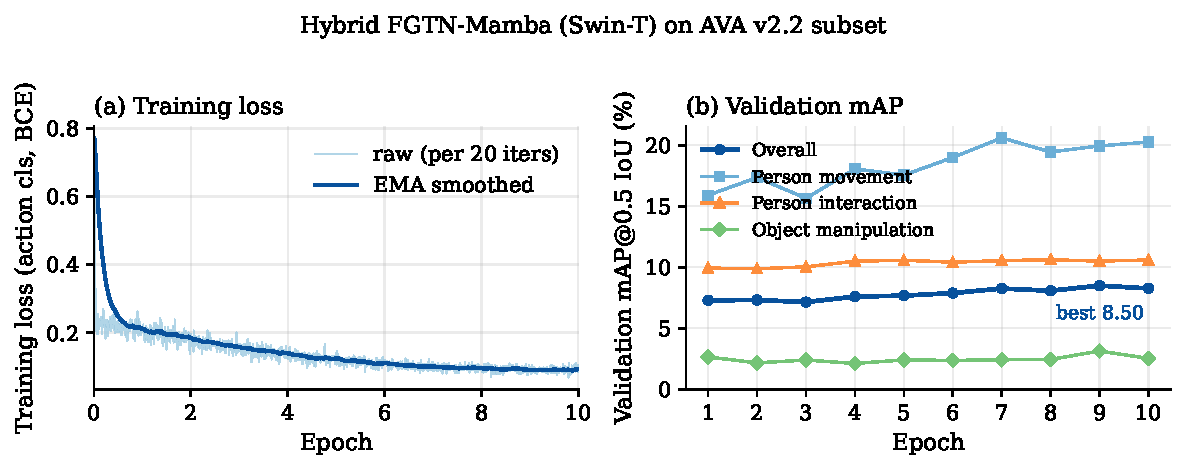
\includegraphics[width=\textwidth]{training_curves.pdf}
\caption[Đường cong huấn luyện và mAP kiểm định trên tập con AVA]{(a) Hàm mất mát huấn luyện (BCE) theo epoch, giá trị thô mỗi 20 iteration và đường làm mượt EMA. (b) mAP kiểm định tổng và theo ba nhóm hành vi; giá trị tốt nhất 8,50\% tại epoch~9. Vẽ từ \code{trainning.log}.}
\label{fig:curves}
\end{figure}

\begin{table}[htbp]
\centering
\caption{Tài nguyên của lần chạy trên tập con AVA với một GPU RTX~4090 (trích từ nhật ký)}
\label{tab:resources}
\begin{tabularx}{\textwidth}{lX}
\toprule
\textbf{Hạng mục} & \textbf{Giá trị}\\
\midrule
Số tham số & 41.827.383 (backbone 27.850.470; neck 13.914.624; head 62.289)\\
Bộ nhớ GPU đỉnh khi huấn luyện & 28.139 MB (epoch~1), 28.800 MB (epoch~2--10), lô 6, FP32\\
Bộ nhớ GPU đỉnh khi kiểm định & 2.058--2.838 MB, lô 1\\
Thời gian một iteration huấn luyện & 0,69--0,70 s (lô 6, gồm nạp dữ liệu 0,02 s)\\
Thời gian một mẫu kiểm định & 0,06--0,08 s (lô 1; $\approx 5{,}8$ phút cho 4.846 khung hình khóa)\\
Tổng thời gian 10 epoch & 5 giờ 55 phút, gồm huấn luyện và kiểm định\\
\bottomrule
\end{tabularx}
\end{table}

Ba nhóm hành vi của AVA có mức hiệu năng khác nhau rõ rệt và ổn định qua các epoch, phản ánh đúng các hạn chế đã nêu ở \cref{sec:gaps}:
\begin{itemize}
  \item \textbf{Chuyển động của người} (15,91\% $\rightarrow$ 20,61\%): tín hiệu toàn thân, bền vững theo thời gian, tương ứng các hành vi trạng thái trong phân xưởng như ngủ trên bàn, gác chân; nhóm được hưởng lợi nhiều nhất từ huấn luyện.
  \item \textbf{Tương tác giữa người} (9,94\% $\rightarrow$ 10,62\%): gần như không đổi sau epoch~4 vì phụ thuộc ngữ cảnh ngoài hộp người (L4), là động cơ tích hợp ACRN.
  \item \textbf{Thao tác với vật thể} (2,12--3,14\%): thấp nhất vì phụ thuộc vật thể nhỏ (L3) và nhiều lớp hiếm (L5), là động cơ cho đặc trưng đa tỉ lệ và hàm mất mát hai cấp; nhóm này cũng chịu ảnh hưởng nặng nhất của sai lệch tỷ lệ RoI dưới đây.
\end{itemize}

\label{sec:roi-stride}\textbf{Sai lệch tỷ lệ RoI.} Khi rà soát mã sau huấn luyện, luận văn phát hiện cấu hình của lần chạy này không đặt \code{featmap\_stride} cho \code{SingleRoIExtractor3D}, nên giá trị mặc định 16 được dùng trong khi tầng 4 của Video Swin-T có bước giảm mẫu 32. Hộp người vì vậy được ánh xạ lên bản đồ đặc trưng ở tỷ lệ gấp đôi: hộp ở nửa phải hoặc nửa dưới ảnh nhận đặc trưng bằng 0, hộp ở góc trên trái nhận đặc trưng của một vùng rộng gấp đôi. Sai lệch không ảnh hưởng tới nhận định về tính ổn định huấn luyện nhưng khiến giá trị mAP tuyệt đối không phản ánh đúng năng lực của cấu hình. Cấu hình một tỉ lệ đã được sửa thành \code{featmap\_stride = 32}; cấu hình đa tỉ lệ dùng 16, đúng với tầng 3 mà mọi bản đồ được nội suy về.

\section{Mốc tham chiếu trên AVA}
\label{sec:reference}

\Cref{tab:reference} liệt kê các mốc công bố trên AVA của những phương pháp ở \cref{ch:related} cùng hai số liệu của luận văn. Các mốc dùng giao thức, backbone và tiền huấn luyện khác nhau nên bảng chỉ cho thấy khoảng hiệu năng của bài toán; số liệu 8,50\% trên tập con không so sánh trực tiếp được với các mốc trên AVA đầy đủ.

\begin{table}[htbp]
\centering
\caption{Mốc công bố trên AVA và kết quả của luận văn (không so sánh trực tiếp; mức bằng chứng E4 cho các hàng tham chiếu)}
\label{tab:reference}
\small
\begin{tabularx}{\textwidth}{>{\raggedright\arraybackslash}p{3.9cm}>{\raggedright\arraybackslash}X>{\raggedright\arraybackslash}p{2.2cm}>{\raggedright\arraybackslash}X}
\toprule
\textbf{Phương pháp} & \textbf{Giao thức} & \textbf{mAP} & \textbf{Ghi chú}\\
\midrule
A* ngoại tuyến \cite{kim2024astar} & AVA v2.2, closed-set & 27,7 & SlowFast-R101-NL, Kinetics-600\\
STAR/CSN-152 \cite{gritsenko2024star} & AVA, end-to-end & 31,4 & IG65M $\to$ K400\\
STAR/B \cite{gritsenko2024star} & AVA, end-to-end & 30,0 & IN21K $\to$ K400\\
STAR/L \cite{gritsenko2024star} & AVA, end-to-end & 39,2 & CLIP $\to$ K700; 320 px\\
OV-STAD \cite{wu2024ovstad} & OV-AVA (base / novel / all) & 27,8 / 16,6 / 25,0 & Open-vocabulary\\
ST-CLIP \cite{huang2025stclip} & ZS-AVA (trung bình; với hộp thật) & 9,01 / 11,76 & Zero-shot\\
\midrule
Hybrid FGTN-Mamba (luận văn, hồ sơ thực nghiệm) & AVA v2.2, closed-set & 39,1 & Swin-T, K400; mức E2; \cref{sec:ava-record}\\
Swin-T + Hybrid FGTN-Mamba một tỉ lệ (luận văn, có nhật ký) & \textbf{Tập con} AVA v2.2, closed-set, \code{featmap\_stride} 16 & 8,50 & K400; 1 GPU; 10 epoch; \cref{sec:ava-subset}\\
\bottomrule
\end{tabularx}
\end{table}

\section{Trả lời câu hỏi nghiên cứu}
\label{sec:rq-answers}

\textbf{RQ1} --- Có cần temporal neck: có; ngay cả MHSA toàn cục tại vị trí hậu-backbone, tiền-RoI cũng tăng mAP ($+3{,}17$ / $+3{,}43$ điểm trên S1 / S2), nhưng Hybrid FGTN-Mamba còn cao hơn neck tiêu chuẩn đó 4,24 / 4,42 điểm. \textbf{RQ2} --- Quét hai chiều có ích ($+1{,}73$ / $+1{,}58$), hai nhánh bổ sung cho nhau ($+1{,}06$ / $+1{,}02$ so với Bi-SSM đứng riêng) và cổng sigmoid đóng góp thêm 1,76 / 1,85 điểm. \textbf{RQ3} --- Đa tỉ lệ cải thiện 3,85 / 2,00 điểm. \textbf{RQ4} --- ACRN cải thiện 5,89 / 3,90 điểm; phần hàm mất mát (A9) chưa có số liệu. \textbf{RQ5} --- Trả lời một phần: mọi thành phần vẫn có ích trên camera chưa thấy khi huấn luyện, với mAP của pipeline đầy đủ giảm từ 89,60\% xuống 78,15\%; số liệu 39,1 mAP trên AVA~v2.2 cần bổ sung cấu hình để đối chiếu.

\section{Hạn chế của nghiên cứu}
\label{sec:limitations}

\begin{itemize}
  \item \emph{Hàm mất mát và độ bất định}: ablation A9 chưa có số liệu; kết quả ablation chưa kèm độ lệch chuẩn giữa các hạt giống; các mô hình so sánh trong \cref{tab:main-results} là lượt chạy đơn, chưa đánh giá trên S2.
  \item \emph{Dữ liệu và tổng quát hóa}: bộ dữ liệu phân xưởng có số camera hạn chế; mAP của pipeline đầy đủ giảm 11,45 điểm khi chuyển sang camera mới; chưa có AP theo từng hành vi.
  \item \emph{Mức bằng chứng}: số liệu trên dữ liệu phân xưởng và 39,1 mAP trên AVA~v2.2 được tổng hợp từ hồ sơ thực nghiệm, nhật ký chi tiết chưa nằm trong kho mã; lần chạy trên tập con AVA còn sai lệch tỷ lệ RoI và learning rate chưa co giãn.
  \item \emph{Khoảng cách tới triển khai}: độ trễ đầu--cuối (gồm bộ phát hiện người và bộ đệm nhìn trước của quét hai chiều) chưa được đo; pipeline vẫn phụ thuộc person proposal và thiết lập closed-set.
\end{itemize}

\section*{Tiểu kết chương}
\addcontentsline{toc}{section}{Tiểu kết chương}

Trên bộ dữ liệu phân xưởng, pipeline đầy đủ đạt 89,83\% mAP và vượt các mô hình so sánh, với tốc độ trên 20 khung hình/giây. Ablation trên hai cách chia dữ liệu xác nhận đóng góp của temporal neck, của hai nhánh, của cổng sigmoid, của đặc trưng đa tỉ lệ và của ACRN; trong đó Hybrid FGTN-Mamba vượt neck tiêu chuẩn tại cùng vị trí hơn 4 điểm trên cả hai cách chia, đáp ứng tiêu chí chấp nhận đã đặt ra. Khoảng cách giữa S1 và S2 cho thấy 78,15\% trên camera mới là ước lượng thận trọng hơn cho triển khai. Các hạn chế về hàm mất mát, độ bất định và mức bằng chứng được nêu rõ để định hướng công việc tiếp theo.

\chapter*{KẾT LUẬN VÀ HƯỚNG PHÁT TRIỂN}
\addcontentsline{toc}{chapter}{KẾT LUẬN VÀ HƯỚNG PHÁT TRIỂN}
\label{ch:conclusion}

\section*{1. Kết luận}

Luận văn đặt ra bài toán phát hiện hành động không--thời gian theo từng người trong bối cảnh giám sát phân xưởng, nơi các hành vi mục tiêu trải trên hai thang thời gian đối lập, và đề xuất Hybrid FGTN-Mamba, một temporal neck lai đặt sau backbone Video Swin-Tiny và trước 3D RoIAlign. Các kết quả chính như sau.

\begin{enumerate}
  \item \textbf{Về thiết kế.} Khối gồm nhánh mô hình không gian trạng thái chọn lọc hai chiều (toàn cục, chi phí tuyến tính theo $T$), nhánh self-attention trong cửa sổ $W = 5$ (cục bộ) và cổng sigmoid học theo từng kênh và từng bước thời gian. Phân tích độ phức tạp cho thấy mọi số hạng đều tuyến tính theo độ dài chuỗi, với phần phụ thuộc cấu trúc thời gian là $O(TC + TWC)$. Vị trí hậu-backbone, tiền-RoI cho phép giữ nguyên trọng số tiền huấn luyện Kinetics-400 và thay thế backbone mà không đổi neck.
  \item \textbf{Về cài đặt.} Khối được cài đặt tự chứa trên MMAction2 (\code{projects/fgtn\_ava}), với bốn chế độ nhánh để ablation, hỗ trợ bản đồ đặc trưng đa tỉ lệ, kèm bản dự phòng thuần PyTorch để kiểm thử trên CPU. Neck hai khối có 13,9 triệu tham số, bằng khoảng một nửa backbone.
  \item \textbf{Về thực nghiệm.} Trên tập con AVA~v2.2 (15.246 khung hình khóa huấn luyện, 4.846 khung hình khóa kiểm định), pipeline đạt frame-mAP@0,5 tốt nhất 8,50\% tại epoch~9 sau 10 epoch trên một GPU RTX~4090, với mAP theo nhóm 19,95\% (chuyển động của người), 10,51\% (tương tác giữa người) và 3,14\% (thao tác với vật thể). Hàm mất mát giảm đơn điệu, mAP kiểm định tăng ổn định và chuẩn gradient hội tụ, cho thấy neck được huấn luyện ổn định trên backbone tiền huấn luyện. Quá trình rà soát mã sau huấn luyện phát hiện bộ trích RoI của lần chạy này dùng tỷ lệ $1/16$ trên bản đồ có bước giảm mẫu 32; sai lệch đã được sửa trong cấu hình và lần chạy cơ sở cần được lặp lại trước khi kết quả được dùng để so sánh với các phương pháp khác.
  \item \textbf{Về các thành phần hỗ trợ.} Đặc trưng đa tỉ lệ (tầng 3 + tầng 4), ACRN và hàm mất mát focal kết hợp trọng số lớp theo số mẫu hiệu dụng đã được cài đặt, kiểm tra về kích thước tensor và tính chất toán học, và tích hợp vào cấu hình huấn luyện cùng ma trận ablation mười hàng.
\end{enumerate}

Các mục tiêu M1, M2 và M3 (\cref{sec:objectives}) đã đạt ở mức thiết kế và cài đặt; M5 đạt một phần với lần chạy cơ sở trên tập con; M4 và các câu hỏi RQ2--RQ5 đã được chuẩn bị đầy đủ nhưng chưa có số liệu.

\section*{2. Hạn chế}

\begin{itemize}
  \item Kết quả chỉ có trên một tập con AVA, một hạt giống, một cấu hình; chưa có ablation để tách đóng góp của từng nhánh.
  \item Lần chạy cơ sở có sai lệch tỷ lệ RoI; kết quả 8,50\% vì vậy là số liệu của cấu hình chưa sửa, không phải số liệu cuối cùng của phương pháp.
  \item Learning rate của công thức 8 GPU được dùng cho một GPU mà không co giãn.
  \item Bộ dữ liệu phân xưởng với bốn hành vi mục tiêu chưa được thu thập và gán nhãn đủ để đánh giá.
  \item Pipeline phụ thuộc person proposal và closed-set; chưa xử lý hành vi mới không có nhãn.
\end{itemize}

\section*{3. Hướng phát triển}

\begin{enumerate}
  \item \textbf{Ngắn hạn (có thể thực hiện với tài nguyên hiện tại):} chạy lại A5 (đã sửa tỷ lệ RoI) với ba hạt giống; chạy A0--A3 để trả lời RQ2; chạy A6--A8 để trả lời RQ3 và RQ4; ghi phân bố cổng $g$ theo epoch để kiểm tra giả thuyết định tuyến dài--ngắn.
  \item \textbf{Trung hạn:} huấn luyện trên AVA~v2.2 đầy đủ với nhiều GPU để so sánh với các mốc công bố; thử nghiệm neck với backbone khác (VideoMAE, MViTv2) để kiểm tra tính độc lập backbone; bổ sung positional bias tương đối cho nhánh cục bộ.
  \item \textbf{Ứng dụng:} thu thập và gán nhãn bộ dữ liệu phân xưởng theo định dạng AVA với phân chia theo camera; tinh chỉnh pipeline; xây dựng chế độ suy luận nhân quả hoặc nhìn trước giới hạn để giảm độ trễ cảnh báo; tích hợp theo dõi (tracking) và logic $m/n$ với cooldown.
  \item \textbf{Dài hạn:} thay person proposal bằng truy vấn end-to-end theo hướng STAR; mở rộng tập lớp bằng căn chỉnh vùng--văn bản (open-vocabulary) trong khi giữ Hybrid FGTN-Mamba làm bộ mô hình hóa thời gian.
\end{enumerate}
\clearpage


% ====================== TÀI LIỆU THAM KHẢO ======================
\clearpage
\phantomsection
\addcontentsline{toc}{chapter}{TÀI LIỆU THAM KHẢO}
\bibliographystyle{IEEEtran}
\bibliography{refs}

% ====================== PHỤ LỤC ======================
\clearpage
\appendix
\titleformat{\chapter}[block]{\centering\bfseries\large}{PHỤ LỤC \thechapter.}{0.5em}{\MakeUppercase}
% Các tệp trong appendix/src/ được build.sh sao chép từ kho mã nguồn trước khi biên dịch.
% Phụ lục đang tắt (\inphulucfalse trong main.tex); phần thân không tham chiếu tới nhãn trong tệp này.

\chapter{Cấu hình huấn luyện}
\label{app:config}

\section{Cấu hình một tỉ lệ dùng cho lần chạy có nhật ký}

So với phiên bản được ghi trong nhật ký, tệp cấu hình hiện tại đã bổ sung \code{featmap\_stride = 32} (\cref{sec:roi-stride}); mọi giá trị khác giữ nguyên. Đường dẫn tệp: \path{projects/fgtn_ava/ava22_swin-tiny_fgtn_32x2x1-10e.py}.
\lstinputlisting[language=Python]{appendix/src/ava22_swin-tiny_fgtn_32x2x1-10e.py}

\section{Cấu hình tập con}
Tệp \path{projects/fgtn_ava/ava22_swin-tiny_fgtn_subset.py}. Nhật ký của lần chạy trên tập con tương ứng với phiên bản \emph{trước} khi tệp này được chỉnh lô 8 / 20 epoch: nhật ký ghi lô 6, 10 epoch và \code{auto\_scale\_lr.enable = False}.
\lstinputlisting[language=Python]{appendix/src/ava22_swin-tiny_fgtn_subset.py}

\section{Cấu hình pipeline đầy đủ (đa tỉ lệ + ACRN + focal/trọng số lớp)}
\lstinputlisting[language=Python]{appendix/src/ava22_swin-tiny_fgtn-ms-acrn-focal_32x2x1-10e.py}

\chapter{Trích đoạn nhật ký huấn luyện}
\label{app:log}

Nhật ký đầy đủ (\code{trainning.log}, 4.847 dòng) được nộp kèm. Dưới đây là phần môi trường và các dòng tổng kết kiểm định của mười epoch, trích nguyên văn.
\lstinputlisting[numbers=none,basicstyle=\ttfamily\scriptsize]{appendix/src/log_excerpt.txt}

\chapter{Mã nguồn khối đề xuất}
\label{app:code}

\section{Hybrid FGTN-Mamba neck}
Tệp \path{projects/fgtn_ava/fgtn_neck.py}.
\lstinputlisting[language=Python]{appendix/src/fgtn_neck.py}

\section{Head focal + trọng số lớp}
Tệp \path{projects/fgtn_ava/heads.py}.
\lstinputlisting[language=Python]{appendix/src/heads.py}

\section{Tính trọng số lớp theo số mẫu hiệu dụng}
Tệp \path{projects/fgtn_ava/make_class_weight.py}.
\lstinputlisting[language=Python]{appendix/src/make_class_weight.py}

\chapter{Bảng truy nguồn số liệu}
\label{app:traceability}

Mỗi con số thực nghiệm trong luận văn được đối chiếu với nguồn trong kho mã hoặc trong hồ sơ thực nghiệm (\cref{tab:trace}). Cột ``Mức'' theo \cref{tab:evidence}.

\begin{longtable}{p{4.2cm}p{2.4cm}p{6.0cm}p{1.0cm}}
\caption{Truy nguồn các số liệu trong luận văn}
\label{tab:trace}\\
\toprule
\textbf{Số liệu} & \textbf{Giá trị} & \textbf{Nguồn} & \textbf{Mức}\\
\midrule
\endfirsthead
\toprule
\textbf{Số liệu} & \textbf{Giá trị} & \textbf{Nguồn} & \textbf{Mức}\\
\midrule
\endhead
mAP pipeline đầy đủ trên dữ liệu phân xưởng & 89,83\% & Hồ sơ thực nghiệm: bảng so sánh mô hình (\cref{tab:main-results}) & E2\\
mAP các mô hình so sánh & \cref{tab:main-results} & Hồ sơ thực nghiệm: bảng so sánh mô hình & E2\\
Precision, Recall tại ngưỡng 0,5 & 81,82\% & Hồ sơ thực nghiệm: đánh giá pipeline đầy đủ & E2\\
Tốc độ xử lý; bộ nhớ GPU & $>$ 20 khung hình/giây; $\approx 10$~GB & Hồ sơ thực nghiệm; điều kiện đo xem \cref{tab:operating} & E2\\
mAP ablation A0--A8 trên S1, S2 & \cref{tab:ablation-results} & Hồ sơ thực nghiệm: bảng tổng hợp ablation, trung bình ba hạt giống & E2\\
mAP trên AVA~v2.2 (hồ sơ) & 39,1 & Hồ sơ thực nghiệm; cấu hình lượt chạy xem \cref{sec:ava-record} & E2\\
mAP tổng tốt nhất (tập con AVA) & 8,50\% (epoch 9) & \code{trainning.log}: dòng ``The best checkpoint with 0.0850 mAP/overall at 9 epoch'' & E1\\
mAP tổng và theo nhóm, 10 epoch & \cref{tab:per-epoch} & \code{trainning.log}: các dòng ``Epoch(val) [k][4846/4846] mAP/overall ...'' & E1\\
Hàm mất mát trung bình mỗi epoch & \cref{tab:per-epoch} & Trung bình 128 giá trị \code{loss} ghi mỗi 20 iteration trong mỗi epoch của \code{trainning.log} & E1\\
Hàm mất mát và chuẩn gradient ban đầu & 0,7704; 2,769 & \code{trainning.log}: dòng ``Epoch(train) [1][20/2541]'' & E1\\
Số iteration mỗi epoch; kích thước lô & 2.541; 6 & \code{trainning.log}: dòng Epoch(train) và \path{train_dataloader.batch_size} trong cấu hình đầu nhật ký & E1\\
Số khung hình khóa kiểm định & 4.846 & \code{trainning.log}: ``Epoch(val) [k][4846/4846]'' & E1\\
Bộ nhớ GPU đỉnh khi huấn luyện / kiểm định & 28.800 MB / 2.838 MB & Trường \code{memory} lớn nhất trong các dòng Epoch(train) / Epoch(val) & E1\\
Thời gian mỗi iteration huấn luyện & $\approx 0{,}70$ s & Trường \code{time} trong các dòng Epoch(train) & E1\\
Thời gian mỗi mẫu kiểm định & $\approx 0{,}07$ s & Trường \code{time} trong các dòng Epoch(val) & E1\\
Thời gian toàn bộ lần chạy & 5 giờ 55 phút & Dấu thời gian đầu (00:20:20) và cuối (06:15:06) của \code{trainning.log} & E1\\
Hạt giống & 397.422.958 & \code{trainning.log}: ``seed: 397422958'' & E1\\
Phần cứng, phiên bản thư viện & \cref{tab:config} & Phần ``System environment'' đầu \code{trainning.log} & E1\\
Siêu tham số neck, tối ưu, lịch lr & \cref{tab:config} & Cấu hình in đầu \code{trainning.log}; tệp cấu hình \cref{app:config} & E1\\
Số tham số từng module & \cref{tab:params} & Tích các kích thước tensor trong danh sách tham số đầu \code{trainning.log} & E1\\
\code{featmap\_stride} của lần chạy trên tập con & 16 & Cấu hình in đầu \code{trainning.log} (không có khóa \code{featmap\_stride}; mặc định của \code{SingleRoIExtractor3D} là 16) & E1\\
Bước giảm mẫu tầng 4 của Swin-T & 32 & Patch $(2,4,4)$ và ba lần gộp patch; \path{fgtn_ava/README.md} ghi $(B, 768, 16, H/32, W/32)$ & E1\\
Số tham số ACRN, neck tầng 3 & $\approx 14{,}6$M; 3,57M & Tính từ kích thước lớp trong \code{ACRNHead} và \code{FGTNNeckAVA(384)} & E1\\
Mốc A*, STAR, OV-STAD, ST-CLIP & \cref{tab:reference} & Bài báo gốc \cite{kim2024astar,gritsenko2024star,wu2024ovstad,huang2025stclip} & E4\\
\bottomrule
\end{longtable}

\chapter{Lệnh tái lập}
\label{app:repro}

Các lệnh dưới đây chạy trên tập con AVA~v2.2 và ánh xạ sang mã cấu hình A0--A9 của \cref{tab:ablation}; với bộ dữ liệu phân xưởng, dùng cùng các khóa ghi đè trên tệp cấu hình của dữ liệu phân xưởng (\canbosung{tên tệp cấu hình dữ liệu phân xưởng}). Chú thích trong liệt kê viết bằng tiếng Anh để tránh lỗi hiển thị dấu của gói \code{listings}.
\begin{lstlisting}[language=bash,numbers=none]
# 1. Environment (GPU machine; see projects/fgtn_ava/README.md)
pip install -U openmim && mim install mmengine "mmcv>=2.0.0,<2.2.0" mmdet "mmaction2>=1.2.0"
pip install causal-conv1d
pip install git+https://github.com/OpenGVLab/video-mamba-suite.git#subdirectory=mamba

# 2. Data: AVA v2.2 subset
bash projects/fgtn_ava/download_ava.sh annotations proposals
python projects/fgtn_ava/make_subset.py --n-train 45 --n-val 8 --seed 42
NUM_JOBS=4 bash projects/fgtn_ava/download_ava.sh videos
CLEAN=1 JPEG_Q=5 bash projects/fgtn_ava/download_ava.sh cut frames

# 3. Single-scale Hybrid FGTN-Mamba (A6), corrected RoI stride.
#    To reproduce exactly the logged run, add --cfg-options
#    model.roi_head.bbox_roi_extractor.featmap_stride=16
CFG=projects/fgtn_ava/ava22_swin-tiny_fgtn_subset.py
mim train mmaction2 $CFG --gpus 1

# 4. Neck ablations: same config, one --cfg-options override each
#    A0: model.neck=None
#    A1: model.neck.branch_mode=attn_only
#        model.neck.window_size=31   (window covers all T=16)
#    A3: model.neck.branch_mode=mamba_only
#    A4: model.neck.branch_mode=attn_only
#    A5: model.neck.branch_mode=no_gate
#    A2 (uni-directional SSM): set bimamba_type="none" in
#        fgtn_neck.py (no config key yet)
mim train mmaction2 $CFG --gpus 1 \
    --cfg-options model.neck.branch_mode=mamba_only    # A3

# 5. Multi-scale + ACRN + focal loss (A8); A7 = A8 without ACRN.
#    Keep the loss identical within a pair (e.g. add
#    model.roi_head.bbox_head.focal_gamma=0.0 to compare with A6).
MS=projects/fgtn_ava/ava22_swin-tiny_fgtn-ms-acrn-focal_subset.py
mim train mmaction2 $MS --gpus 1                         # A8
mim train mmaction2 $MS --gpus 1 \
    --cfg-options model.roi_head.shared_head=None        # A7

# 6. Loss ablation on A8 (A9). Focal only = the A8 run above;
#    BCE: focal_gamma=0.0; class weights: class_weight=$W.
#    Set class_weight on the head key: a top-level class_weight=...
#    override is ignored (the config resolves it at load time).
python projects/fgtn_ava/make_class_weight.py \
    --ann data/ava/annotations/ava_train_v2.2_subset.csv \
    --out data/ava/annotations/class_weight_train_subset.json
W=data/ava/annotations/class_weight_train_subset.json
# focal + class weights
mim train mmaction2 $MS --gpus 1 \
    --cfg-options model.roi_head.bbox_head.class_weight=$W

# 7. CPU self-check (no mmaction / GPU required)
python projects/fgtn_ava/selfcheck.py
\end{lstlisting}


\end{document}
